%  LaTeX support: latex@mdpi.com
%  For support, please attach all files needed for compiling as well as the log file, and specify your operating system, LaTeX version, and LaTeX editor.

%=================================================================
\documentclass[journal,article,submit,pdftex,moreauthors]{Definitions/mdpi}
% For posting an early version of this manuscript as a preprint, you may use "preprints" as the journal and change "submit" to "accept". The document class line would be, e.g., \documentclass[preprints,article,accept,moreauthors,pdftex]{mdpi}. This is especially recommended for submission to arXiv, where line numbers should be removed before posting. For preprints.org, the editorial staff will make this change immediately prior to posting.


%=================================================================
% MDPI internal commands
\firstpage{1}
\makeatletter
\setcounter{page}{\@firstpage}
\makeatother
\pubvolume{1}
\issuenum{1}
\articlenumber{0}
\pubyear{2022}
\copyrightyear{2022}
%\externaleditor{Academic Editor: Firstname Lastname}
\datereceived{}
%\daterevised{} % Only for the journal Acoustics
\dateaccepted{}
\datepublished{}
%\datecorrected{} % Corrected papers include a "Corrected: XXX" date in the original paper.
%\dateretracted{} % Corrected papers include a "Retracted: XXX" date in the original paper.
\hreflink{https://doi.org/} % If needed use \linebreak
%\doinum{}
%------------------------------------------------------------------
% The following line should be uncommented if the LaTeX file is uploaded to arXiv.org
%\pdfoutput=1

%=================================================================
% Add packages and commands here. The following packages are loaded in our class file: fontenc, inputenc, calc, indentfirst, fancyhdr, graphicx, epstopdf, lastpage, ifthen, lineno, float, amsmath, setspace, enumitem, mathpazo, booktabs, titlesec, etoolbox, tabto, xcolor, soul, multirow, microtype, tikz, totcount, changepage, attrib, upgreek, cleveref, amsthm, hyphenat, natbib, hyperref, footmisc, url, geometry, newfloat, caption

%=================================================================
%% Please use the following mathematics environments: Theorem, Lemma, Corollary, Proposition, Characterization, Property, Problem, Example, ExamplesandDefinitions, Hypothesis, Remark, Definition, Notation, Assumption
%% For proofs, please use the proof environment (the amsthm package is loaded by the MDPI class).

\usepackage{algorithm}
\usepackage{algorithmic}

\graphicspath {{./fig/}}

%\usepackage{amsmath} % assumes amsmath package installed
\usepackage{amssymb}  % assumes amsmath package installed
\usepackage{amsthm}  % assumes amsmath package installed
\usepackage{amsmath}  % assumes amsmath package installed

\usepackage{url}

\usepackage{changes} %宏包
\definechangesauthor[name={Lin Li}, color=red]{Lin} % 设置批注人的名字

%=================================================================
% Full title of the paper (Capitalized)
\Title{Exact and Heuristic Multi-robot Dubins Coverage Path Planning for known environments }

% MDPI internal command: Title for citation in the left column
\TitleCitation{Title}

% Author Orchid ID: enter ID or remove command
\newcommand{\orcidauthorA}{0000-0000-0000-000X} % Add \orcidA{} behind the author's name
%\newcommand{\orcidauthorB}{0000-0000-0000-000X} % Add \orcidB{} behind the author's name

% Authors, for the paper (add full first names)
\Author{Lin Li$^{1}$\orcidA{}, Dianxi Shi $^{2, 3}$*, Songchang Jin $^{2,3}$*, Shaowu Yang $^{1}$*, Chenlei Zhou $^{3}$, Yaoning Lian$^{1}$, and Hengzhu Liu$^{1}$}
%\Author{XX XX$^{1,\dagger,\ddagger}$\orcidA{}, XX XX $^{2,\ddagger}$ and XX XX $^{2,}$*}
% zhouchenlei58@126.com

%\longauthorlist{yes}

% MDPI internal command: Authors, for metadata in PDF
\AuthorNames{Firstname Lastname, Firstname Lastname and Firstname Lastname}

% MDPI internal command: Authors, for citation in the left column
\AuthorCitation{Lastname, F.; Lastname, F.; Lastname, F.}
% If this is a Chicago style journal: Lastname, Firstname, Firstname Lastname, and Firstname Lastname.

% Affiliations / Addresses (Add [1] after \address if there is only one affiliation.)
\address{%
$^{1}$ \quad College of Computer, National University of Defense Technology, Changsha, China.\\
$^{2}$ \quad Artificial Intelligence Research Center (AIRC) Defense Innovation Institute, Beijing, China.\\
$^{3}$ \quad Tianjin Artificial Intelligence Innovation Center (TAIIC), Tianjin, China.}

% Contact information of the corresponding author
\corres{Correspondence: dianxishi@nudt.edu.cn, jsc04@tsinghua.org.cn}
%\corres{Correspondence: dianxishi@nudt.edu.cn, dianxishi@nudt.edu.cn; Tel.: (optional; include country code; if there are multiple corresponding authors, add author initials) +xx-xxxx-xxx-xxxx (F.L.)}

% Current address and/or shared authorship
%\firstnote{Current address: Affiliation 3.}
%\secondnote{These authors contributed equally to this work.}
% The commands \thirdnote{} till \eighthnote{} are available for further notes

%\simplesumm{} % Simple summary

%\conference{} % An extended version of a conference paper

% Abstract (Do not insert blank lines, i.e. \\)
\abstract{ \added{Coverage path planning (CPP) of multiple Dubins robots has been extensively applied in aerial monitoring, marine exploration, and search and rescue.} Existing multi-robot coverage path planning (MCPP) works use exact or heuristic algorithms to address coverage applications. However, several exact algorithms always provide precise area division rather than coverage paths, and heuristic methods face the challenge of balancing accuracy and complexity. This paper focuses on the \added{Dubins} MCPP problem \replaced{of known environments}{for multiple Dubins robots}. Firstly, we present an \replaced{exact Dubins MCPP (EDM)}{EMD} algorithm \replaced{based on}{modelling the MCPP problem as} mixed linear integer programming (MILP). The EDM algorithm \replaced{ searches the entire solution space to obtain the shortest Dubins coverage path.}{provides precise coverage paths by simultaneously optimizing task allocation and path planning subproblems.} Secondly, a heuristic approximate \replaced{credit-based Dubins MCPP (CDM)}{CMD} algorithm is presented, which utilizes the credit model to balance tasks among robots and a tree partition strategy to reduce complexity. Comparison experiments with other exact and approximate algorithms demonstrate that \replaced{EDM}{EMD} provides the least coverage time in small scenes, and \replaced{CDM}{CMD} produces shorter coverage time and less computation time in large scenes. Feasibility experiments demonstrate the applicability of \replaced{EDM}{EMD} and \replaced{CDM}{CMD} to a high-fidelity fixed-wing unmanned aerial vehicle (UAV) model.}



% Keywords
\keyword{complete coverage, Dubins robot, path planning}


%%%%%%%%%%%%%%%%%%%%%%%%%%%%%%%%%%%%%%%%%%
\begin{document}

%%%%%%%%%%%%%%%%%%%%%%%%%%%%%%%%%%%%%%%%%%
\setcounter{section}{-1} %% Remove this when starting to work on the template.

\section{Introduction}

\added{As one subproblem of robot path planning,} coverage path planning (CPP) \replaced{aims to determine}{is the task of determining} a path to visit all points in the region \cite{fevgas2022coverage}. \replaced{CPP is common to several applications, including}{Various robotic applications requiring CPP include} small-scale household tasks like floor cleaning or lawn mowing and large-scale operations like search and rescue and environmental monitoring \cite{c46}. \added{Due to the limited sensing range, calculating speed, and energy supply, many practical coverage applications cannot be achieved by a single robot \cite{chen2021clustering}. Thus, a series of multi-robot CPP (MCPP) algorithms have been proposed to improve coverage efficiency and enhance robustness. Meanwhile, MCPP faces the challenges of algorithmic complexity and logistical management \cite{c16}.} \deleted{ The CPP problem's complexity depends on factors such as the complexity of the environments, and the kinematic constraints of robots \cite{lewis2017semi}. In general, a robot with nonholonomic constraints is more challenging to plan than one with holonomic constraints \cite{wang2017curvature}, and an obstacle-constrained environment is more involved in planning than one without obstacles \cite{c2}.}

\added{Real-world MCPP applications, such as aerial monitoring \cite{coombes2019flight}, marine exploration\cite{wilson2019novel}, and automatic farming \cite{maini2022online}\cite{c11}, typically involve multiple aerial (fixed-wing aircraft), ground (wheel robots), and autonomous underwater/surface vehicles. These vehicles are typically governed by the Dubins vehicle model \cite{dubins1957curves}, which allows them to move at a fixed speed and turn with a limited turning radius. As the foundation of many practical applications, MCPP oriented to Dubins robots (Dubins MCPP) has received growing attention in recent years. Thus, this paper focuses on the Dubins MCPP problem of known environments.}

%\added{Typical applications like marine monitoring or requires} Since Dubins robots are widely used in practical applications, including automatic farming \cite{c12}, field  exploration, and area exploration \cite{wilson2019novel}, the CPP problem of Dubins robots has received increasing attention.

% As the foundation of many robotic applications,  Roughly, the complexity of the CPP problem is determined by factors such as the complexity of coverage environments and the kinematic constraints of robots \cite{lewis2017semi}. Depending on their scales, coverage environments can be classified as small (e.g., floor cleaning and lawn mowing) or large (e.g., environmental monitoring \cite{c6}) \cite{karapetyan2018multi}. Based on kinematic constraints, coverage robots can be divided into holonomic and nonholonomic robots \cite{khan2017complete}. As one of the classic nonholonomic constraint robots, Dubins robots have received increasing attention in recent years since they are widely used in practical applications, such as automatic agriculture \cite{c12}, search and rescue, and area exploration \cite{c2}. Thus, this paper addresses the CPP problem for known environments with Dubins robots.

\deleted{Utilizing multiple robots can reduce coverage time and increase robustness \cite{munoz2021multi}. However, multi-robot CPP (} MCPP problem has been proven to be NP-hard \cite{rekleitis2008efficient}. Various MCPP works have been proposed to address the MCPP problem, and the related reviews can be found in \cite{c29}\cite{c30}\cite{c31}. Existing MCPP methods can be classified as exact or heuristic according to their accuracy \cite{yu2020balanced}. Exact methods can provide the optimal solution for small-scale coverage applications. Heuristic methods are used to get a (near-) optimal result for large-scale coverage applications since they often involve a great number of tasks.

% decompose the MCPP into task allocation and path planning subproblems. However, the combinational solution of subproblems is not optimal for MCPP.
Existing MCPP methods perform well, but they suffer from three issues. The first issue is that several exact methods always provide an accurate partition of the region. However, the accurate partition is not equivalent to optimal coverage paths for the MCPP problem. Second, heuristic methods always face the challenge of how to balance accuracy and complexity. Traditional heuristic methods represent coverage tasks as graphs and obtain an efficient result using graph-partition and tree-partition strategies. In the graph-partition strategy, all vertexes and edges are considered to achieve near-optimal results. However, its runtime increases since the search space increase exponentially with the number of vertexes \cite{yu2020balanced}. The tree-partition strategy compresses the search space of the MCPP problem by pruning the edges of the graph. While the compressed search space reduces the runtime, it decreases the accuracy of the solution. The third issue is that many MCPP works have been proposed, but only a few studies have been conducted on the Dubins robot. As a curvature-constrained robot, the Dubins robot cannot recede and can only move at a fixed speed and with a bound curvature. Without consideration of robot kinematics, MCPP algorithms probably generate piecewise paths that are only comprised of straight lines and sharp turns \cite{khan2017complete}. However, these paths are not feasible to follow for Dubins robots.

% formulate the problem into a set of Mixed Integer Linear Programming (MILP) models

This paper presents two algorithms to address the \replaced{Dubins MCPP}{multi-robot Dubins CPP (MDCPP)} problem. First, an exact \replaced{Dubins MCPP (EDM)}{multi-robot Dubins CPP (EMD}) algorithm is proposed, formulating the Dubins MCPP problem as a MILP to produce the optimal Dubins coverage paths. Second, we present a heuristic approximate credit-based \deleted{ multi-robot} Dubins MCPP \replaced{(CDM)}{CMD} algorithm. \replaced{CDM}{CMD} divides the region into multiple partitions by a tree-partition strategy and balances coverage tasks among partitions by the credit model \cite{li2022complete}. The effectiveness of \replaced{EDM}{EMD} and \replaced{CDM}{CMD} was validated in comparison and feasibility experiments. In summary, the contributions of this paper are as follows:
\begin{itemize}
\item We present an \replaced{EDM}{EMD} algorithm \replaced{based on MILP, which provides the shortest Dubins coverage path by searching the entire solution space.}{ modeling the MCPP problem as MILP.}
\item We present a \replaced{CDM}{CMD} algorithm, which ensures the task balance among robots by the credit model and reduces complexity by a tree-partition strategy.
\item Extensive validations. (i) Comparison experiments with other exact and heuristic MCPP methods show that \replaced{EDM}{EMD} provides the minimum coverage time in small coverage scenes, and \replaced{CDM}{CMD} generates a shorter coverage time and less computation time in large coverage scenes. (ii) Feasibility experiments are conducted on a high-fidelity UAV model to validate the applicability of \replaced{EDM}{EMD} and \replaced{CDM}{CMD}.
\end{itemize}

The remaining of this paper is organized as follows. In Section \ref{Sec_Related_Work}, the related works are reviewed. Section \ref{Sec_Problem_Statement} states the \replaced{Dubins MCPP}{DMCPP} problem and presents a Dubins coverage framework. Section \ref{Sec_EMD} and \ref{Sec_CMD} describe \replaced{EDM}{EMD} and \replaced{CDM}{CMD}, including their ideas and implementation. The comparison and feasibility tests of \replaced{EDM}{EMD} and \replaced{CDM}{CMD} are presented in Section \ref{Sec_Experiments}, followed by the paper's conclusion.

\section{Related Work}
\label{Sec_Related_Work}

\subsection{Exact and heuristic MCPP methods}

Existing works use exact and heuristic algorithms to solve the MCPP problem. Exact algorithms guarantee an optimum solution, while heuristic algorithms seek to yield a good, but not necessarily optimal, solution. However, an exact algorithm takes much longer to find an optimum solution than a heuristic one to a difficult problem \cite{Rafael2022Exact}. Thus, exact algorithms are suitable for small-scale applications, whereas large-scale coverage applications often use heuristics to achieve a suboptimal solution.

Exact MCPP algorithms use the MILP \cite{c39}\cite{matic2014mixed}, branch and bound method \cite{sundar2017algorithms}, and dynamic programming method to obtain the optimum solution. \added{Some exact algorithms precisely divide the region into $K$ partitions and apply a single-robot coverage algorithm to each partition.} For example, the work \deleted{\cite{chlebikova1996approximating} proves that $BCP_q$ is NP-hard and proposes a polynomial-time algorithm that solves $BCP_2$ within an approximation ratio of $\frac{4}{3}$. \cite{matic2014mixed} proposes an accurate MILP for two robots, which can solve graphs of 70 nodes within two hours. However, the MILP is difficult to extend to cases with $q \geq 3$. The work } \cite{c39} transforms the MCPP problem into \added{the $MinMax$ balanced and connected $q$-partition problem (}$BCP_q$\added{)} and presents an exact Milpflow algorithm to handle it. The Milpflow algorithm provides a precise partition of the region through a flow model and applies a single-robot CPP algorithm to each partition. However, the optimial partition is not equivalent to optimal coverage paths. \added{Other exact works build exact formations based on MILP to generate the shortest or fastest paths.} For example, the works \added{\cite{chen2021clustering}\cite{yu2020balanced} produces the fastest coverage paths by building exact formulations. However, both works calculate the coverage time of a given region based on the scanning area rather than the coverage path. In fact, the coverage time of a given region depends on the time to cover the scanning area and the time to perform turns. Since turns are often costly for mobile robots, neglecting the cost of turns usually reduces the efficiency \cite{vandermeulen2019turn}. In order to minimize the cost of turns, the work \cite{yu2015optimization} divides the region into cells and represents cells as a graph. The Dubins MCPP problem is formulated with the graph representation as a generalized traversal salesman problem (TSP). The exact coverage path is then obtained by applying the GTSP solver. Unfortunately, the work \cite{yu2015optimization} is only applicable to a single robot.} \deleted{proposed an exact formulation to address the coverage problem for scattered regions. This formulation model MCPP as a $MinMax$ problem for balancing robot coverage times. However, this formulation does not apply to practical coverage applications since it does not consider robot kinetics. Several works models the optimal coverage problem as the $MinMax$ balanced and connected $q$-partition problem ($BCP_q$) and present various methods to resolve it.}

Heuristic MCPP algorithms usually decompose the region into cells and represent them in a graph. With the graph representation, graph-partition and tree-partition strategies are utilized to divide the graph into multiple parts. Each part corresponds to one robot. The graph-partition strategy takes all information of the graph into account to obtain a (near-) optimal result. For example, to address the area patrolling problem of heterogeneous robots, the work \cite{c41} utilizes the auction algorithm to assign appropriate tasks to robots. Although the auction algorithm has the advantage of low complexity, its greedy strategy leads to local-optimal allocation. The authors in \cite{li2022complete} extend the traditional market-based methods and propose a credit-based task allocation (CTA) algorithm. The CTA algorithm balances the tasks among robots by a credit model and reduces complexity by transforming a multi-objective optimization problem into a set of single-objective optimization problems. However, the CTA algorithm is unsuitable for coverage applications relying on Morse or BCD decomposition since it assumes that coverage tasks are uniform grids. In \cite{c46}, two heuristics algorithms are presented to address the MCPP problem for known environments. The first algorithm calculates the Eulerian tour of visiting all tasks and produces $ k$ subtours by a k-postman approximation algorithm. The second one uses a greedy approach that divides the area into equal regions, covering each region with a single robot. Although the graph-partition strategy performs well, it has long runtime for graphs with a significant number of vertexes and edges.

The tree partition strategy reduces the runtime by deleting edges from the graph. However, some optimality is sacrificed since the search space shrinks after edge deletion. In \cite{gabriely2001spanning}, the authors proposed a spanning tree coverage (STC) algorithm for single robots. The STC algorithm incrementally builds a virtual tree and navigates the robot around the tree to achieve complete coverage. The work \cite{hazon2005redundancy} extends the STC algorithm and presents a multi-robot STC algorithm, which reduces coverage time by two times while no repeated tasks are generated. Nevertheless, it cannot guarantee an optimal result with the rise of robots. Literature \cite{zheng2005multi} proposed a polynomial-time algorithm that assigns tasks to $k$ robots by finding a weighted tree of $k$ ($k =$ number of robots) covering all nodes. The polynomial-time algorithm ensures that its coverage time is eight times the optimal coverage time. However, it assumes that the trees can be overlapped. The genetic algorithm was also used to solve the tree partition problem due to its excellent performance. In the genetic algorithm, each individual is composed of a forest of non-intersecting trees, and the population evolves to find the (near-) optimum. For example, the work \cite{c39} presented a genetic algorithm based on tree partition and evolution. The genetic algorithm can handle graphs with up to 3000 nodes.\cite{c1} presents an algorithm called mofint for finding the least number of robots within a time limit. The mofint algorithm transforms the time-limit version of MCPP into a bi-objective optimization problem and applies a multi-objective genetic method. Although genetic algorithms perform well, they often produce local optimal solutions due to their evolutionary operations.

\subsection{Dubins coverage}
The exact and heuristic MCPP methods provide optimal or near-optimal paths that visit all points of the region. However, due to their lack of consideration of robot kinematics, several MCPP methods could not guarantee the path's curvature continuity. Curvature discontinuities threaten robot safety and degrade the robots' dead-reckoning abilities \cite{wang2017curvature}\cite{vselek2022smooth}. Thus, the construction of feasible and smooth paths has received much attention in robotic research fields \cite{khan2017complete}.

% To address the problem of finding the shortest path for robots with a single forward speed and a maximum turning radius in open areas.

The Dubins path \cite{dubins1957curves} provides the shortest path for robots with a single forward speed and a maximum turning radius in open areas. As Dubins paths can be expressed analytically and are quickly computed, a series of Dubins coverage methods based on them were presented. Dubins coverage has numerous practical applications, such as automated agriculture \cite{c12}, search and rescue, and seabed inspection. For example, the authors in \cite{xu2011optimal} presented a coverage algorithm for a fixed-wing unmanned aerial vehicle (UAV). The coverage algorithm breaks the region into multiple subcells and produces the Eulerian circuit with minimum path repetition. The effectiveness of the proposed algorithm \cite{xu2011optimal} has been validated in field trials. The authors in \cite{yu2015optimization} modelled the Dubins coverage problem into an generalized traversal salesman problem (GTSP). The coverage path with the lowest non-working travel is obtained by transforming the GTSP into an asymmetry traversal salesman problem (ATSP). By re-setting the path cost between two points separated by obstacles, the work \cite{yu2015optimization1} extended \cite{yu2015optimization} to non-convex environments. The work \cite{lewis2017semi} proved that the optimal Dubins coverage problem is NP-complete and presents a coverage algorithm for single Dubins robot. In \cite{karapetyan2018multi}, the authors present two heuristics methods called DCRC and DCAC for addressing the CPP problem with multiple Dubins vehicles. DCRC generates an optimal Hamiltonian path and uses the route clustering to divide the path into $K$ subpaths. DCAC divides the area into multiple partitions and applies the single-robot Dubins solver \cite{lewis2017semi} to each subarea. The simulation results in \cite{karapetyan2018multi} show that DCRC has better performance than DCAC.

\section{System Overview}
\label{Sec_Problem_Statement}

This section describes related definitions of the \replaced{Dubins MCPP}{MDCPP} problem and presents a Dubins coverage framework.

\subsection{Problem Statement}
\label{subsec_Problem_Statement}
We assume to have $K$ homogeneous Dubins robots to perform the coverage task. All robots constitute a robot set $R = \{r_1,...,r_K\}$. The Dubins robots in $R$ are equipped with the same task sensor for specific tasks (e.g., cleaning the floor or detecting objects). The task sensor can cover a rectangular area of $w_1$ in width. All robots start from the same starting point $p_s$ and travel at a fixed speed $s$ with a minimum turning radius $r$.

\begin{figure}[htb] %这里使用的是强制位置,除非真的放不下,不然就是写在哪里图就放在哪里,不会乱动
	\centering  %图片全局居中
    \vspace{0 cm} %设置与上面正文的距离
    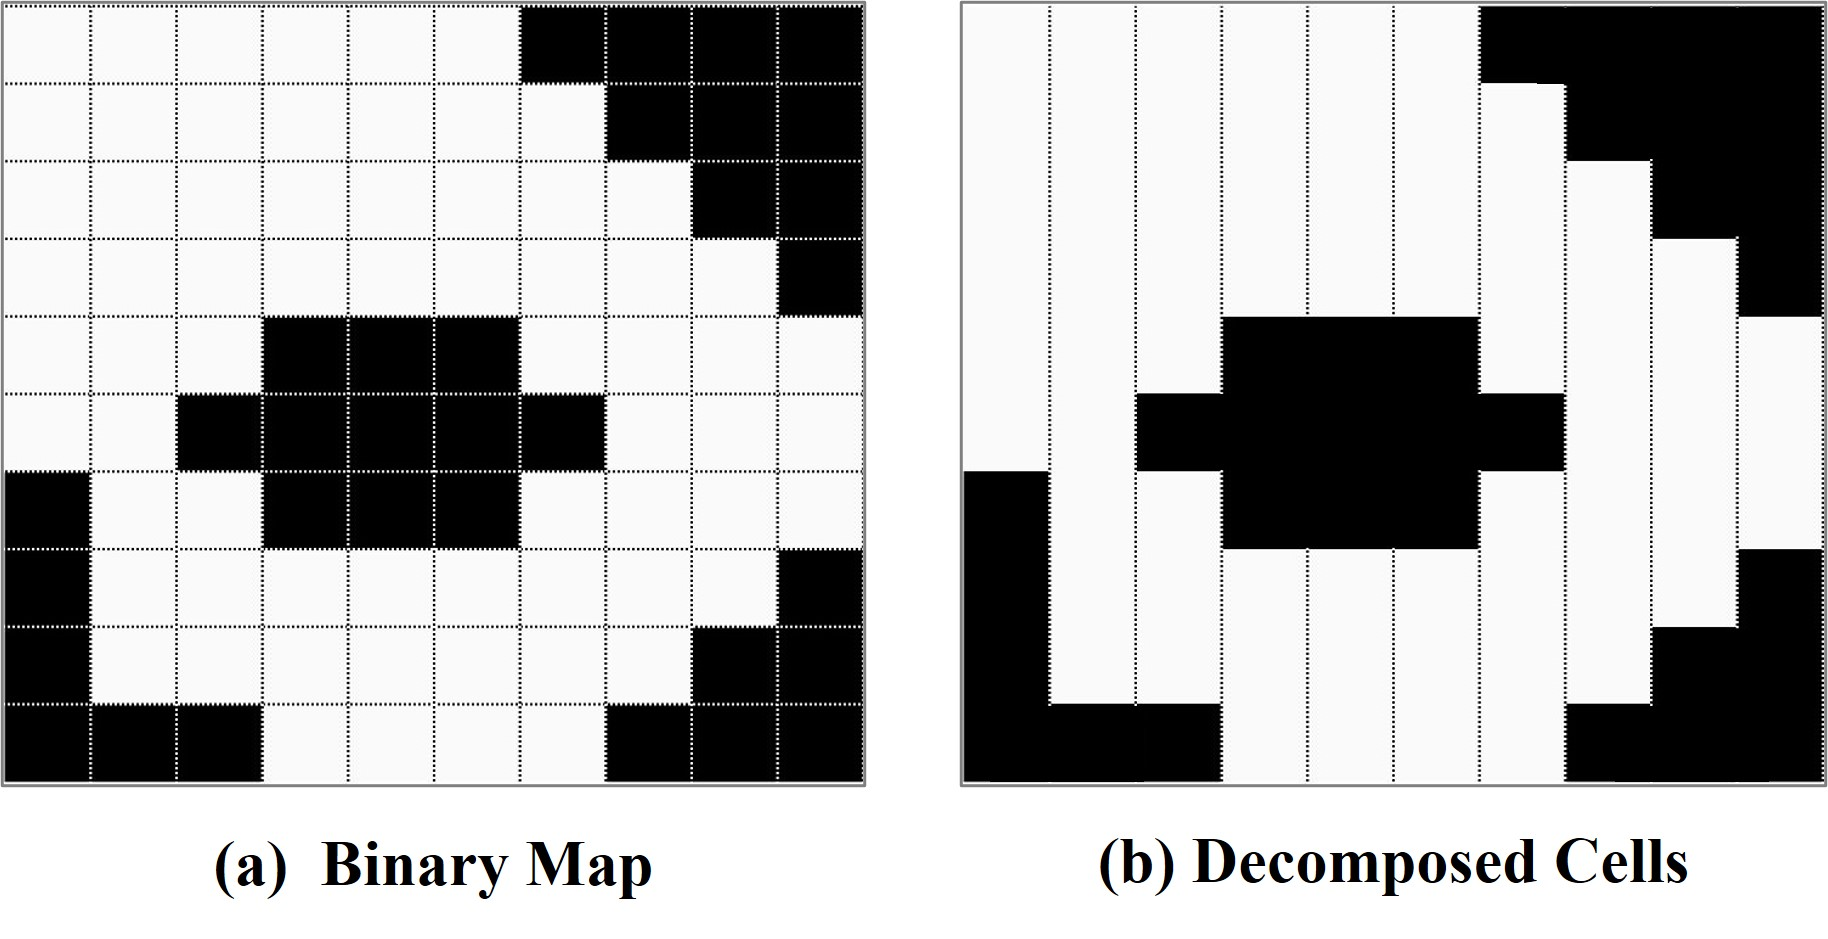
\includegraphics[width=0.6\textwidth]{1.jpg}
    \caption{ Decomposing the mission environment into cells.}
%    \vspace{-0.2 cm} %设置与下面正文的距离
   \label{Fig_area_decomposition}
\end{figure}

The mission environment is assumed to be known and has been represented as a binary map. In this binary map, cells with values of 0 or 1 represent obstacles or allowed areas, respectively. To avoid being restricted to one kind of robot model, classical Dubins approaches \cite{c46}\cite{c56} assume that obstacles are areas that are not necessarily covered but can be crossed. Similarly, this paper assumes that the robot can cross the obstacle. The semi-BCD decomposition \cite{c56} method is used to divide the region into $N$ rectangular cells. All cells form the set of cells $C =\{ c_1,...,c_n,...,c_N\}$, where $c_n$ represents the $n$-th cell in $C$. Each cell has a width of $w_1$, and its height depends on the boundary of the region and obstacles. Fig.~\ref{Fig_area_decomposition} represents an example of area decomposition.

The objective of MDCPP is to produce a path for each robot so that every point of the allowed areas is covered at least by one robot. Since all robots have the same kinetic constraints, an efficient solution is to minimize robot path lengths while equally distributing robot workloads. Hence, \replaced{Dubins MCPP}{MDCPP} can be viewed as a $MinMax$ problem, i.e., to minimize the maximum cost of all robots.

\subsection{System Overview}

\begin{figure}[bp] %这里使用的是强制位置,除非真的放不下,不然就是写在哪里图就放在哪里,不会乱动
	\centering  %图片全局居中
    \vspace{0 cm} %设置与上面正文的距离
    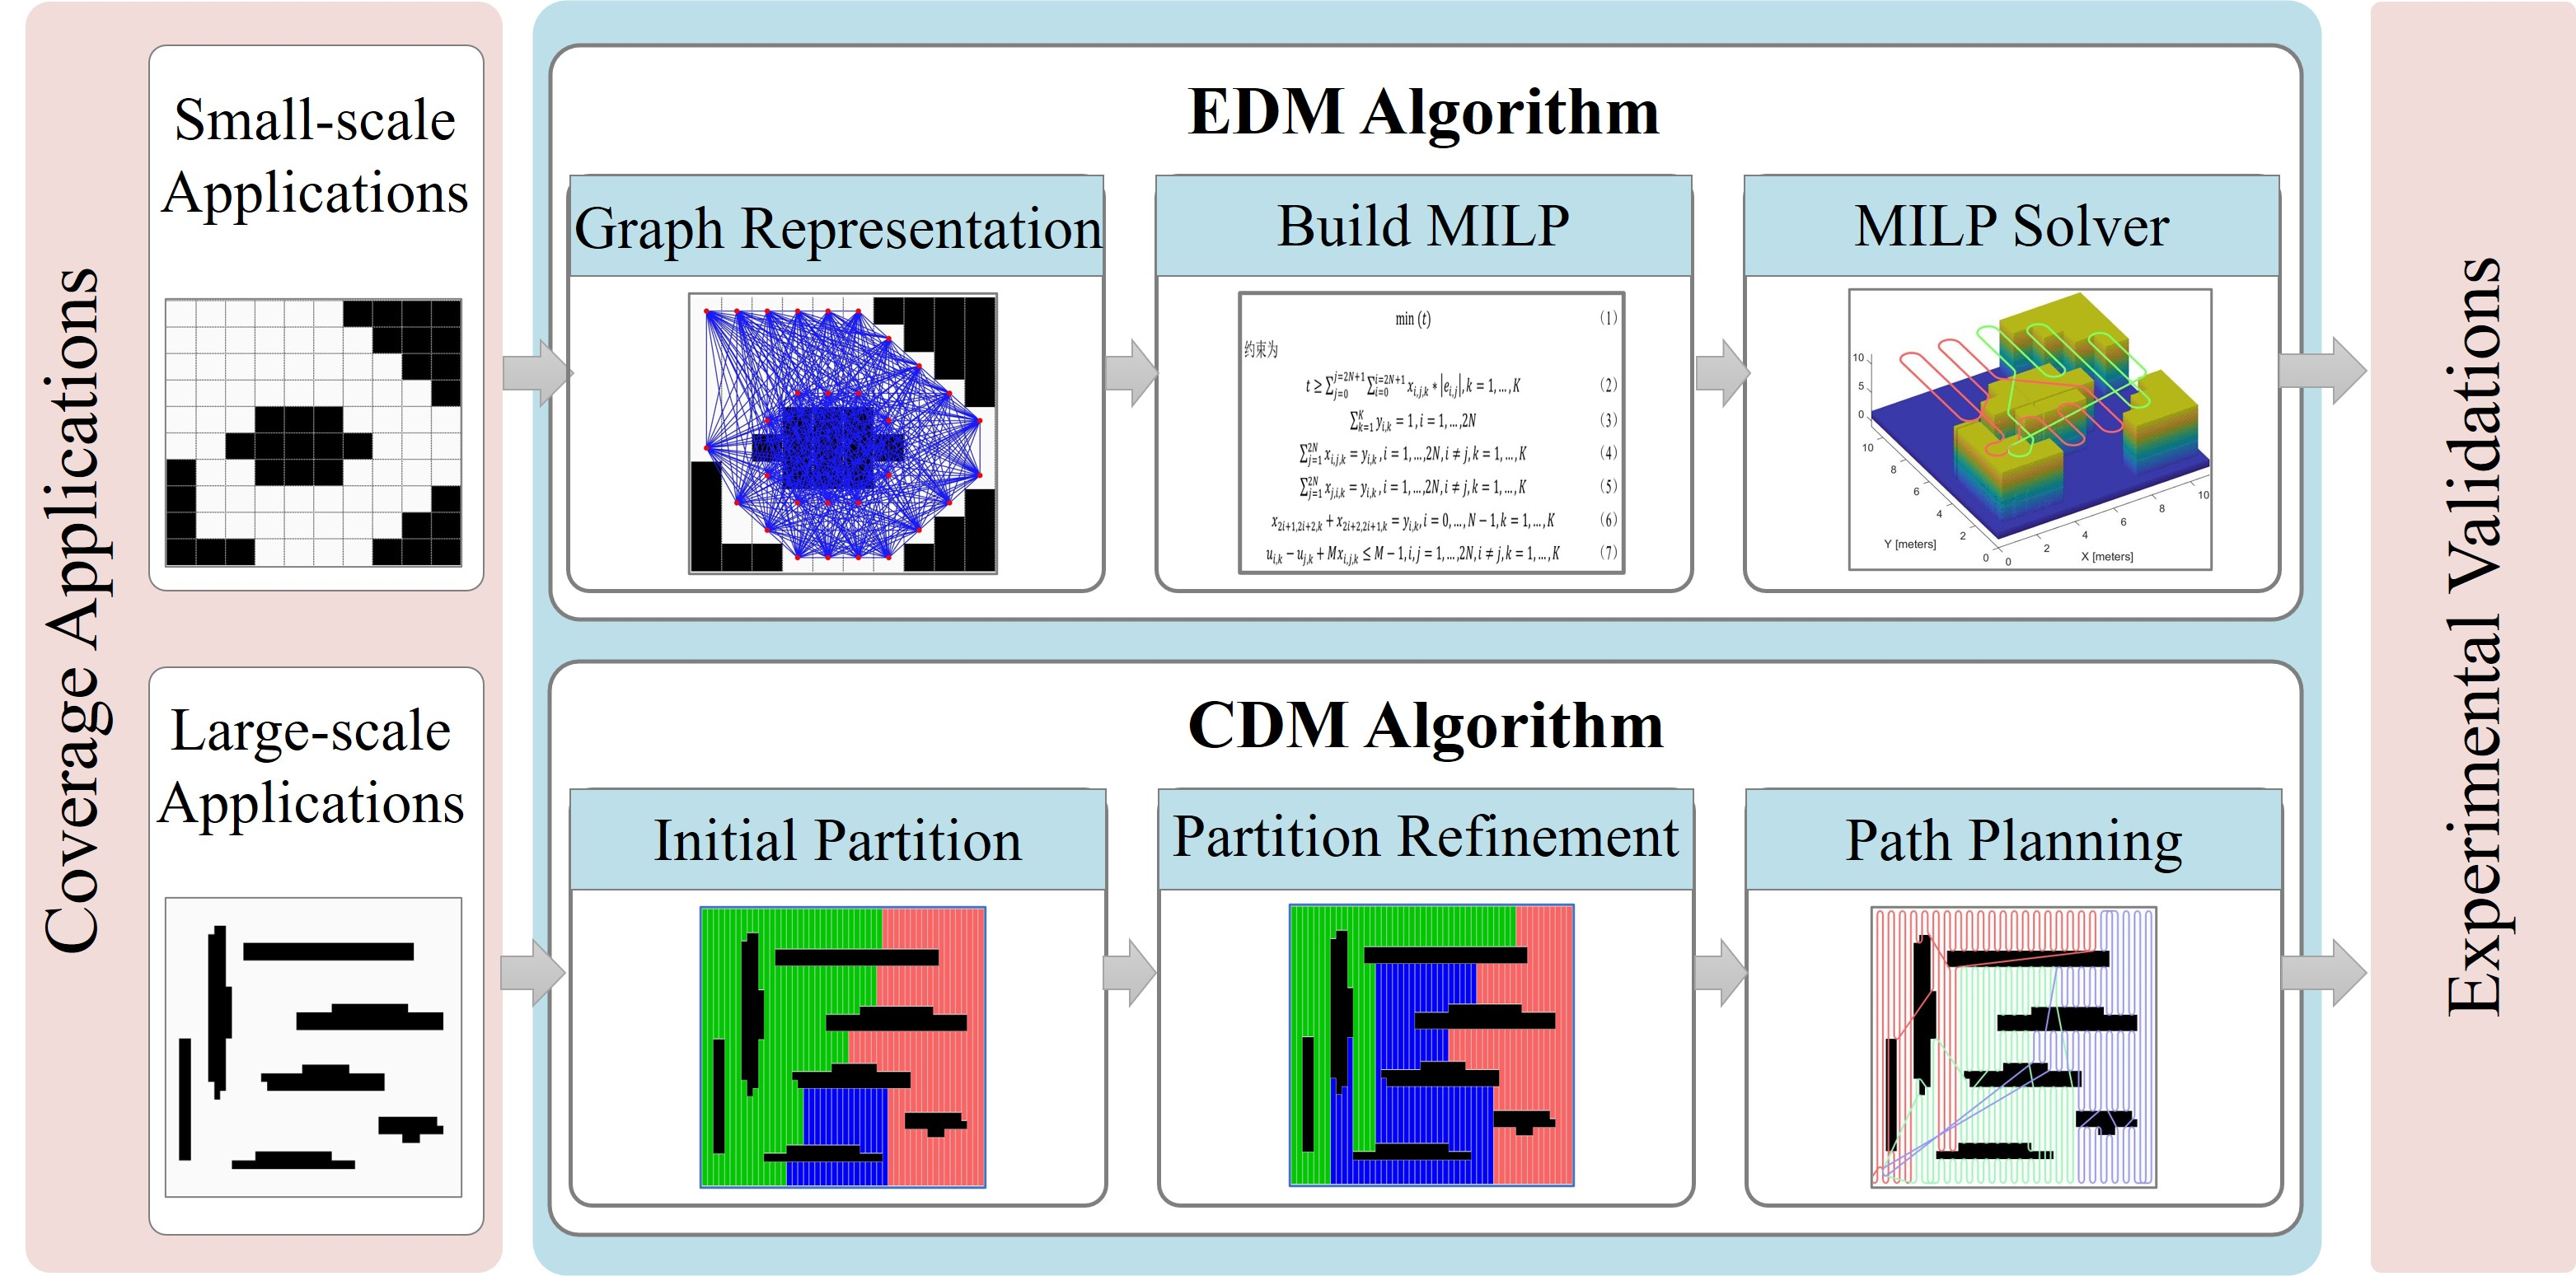
\includegraphics[width=0.95\textwidth]{10.jpg}
    \caption{ An overview of the Dubins coverage framework.}
 %   \vspace{-0.2 cm} %设置与下面正文的距离
   \label{Fig_framework}
\end{figure}

This paper presents a Dubins coverage framework to address the \replaced{Dubins MCPP}{DMCPP} problem. As shown in Fig.\ref{Fig_framework}, the framework comprises coverage applications, \replaced{Dubins MCPP}{DCMPP} methods, and experimental validations. The component of the \replaced{Dubins MCPP}{DMCPP} methods consists of an \replaced{EDM}{exact EMD} algorithm and a heuristic \replaced{CDM}{CMD} algorithm. \replaced{The EDM algorithm}{EMD} represents coverage tasks as a graph and \replaced{proposes an exact formation based on MILP. The MILP solver is used to produce the optimal Dubins coverage path by thoroughly searching the solution space.}{builds a MILP to obtain the optimal Dubins coverage paths.} \replaced{The CDM algorithm}{CMD} divides the region into $K$ subareas through initial partition and partition refinement modules. The single-robot Dubins solver \cite{c25} is then employed in each subarea. More details of \replaced{EDM}{EMD} and \replaced{CDM}{CMD} are presented in Section \ref{Sec_EMD} and \ref{Sec_CMD}.

\section{Exact \replaced{Dubin Multi-robot CPP (EDM)}{Multi-robot Dubin CPP (EMD)} Algorithm}
\label{Sec_EMD}

Exact methods \replaced{either provide an accurate partition or produce coverage paths without considering the turning cost of the robot covering a given region, resulting in a non-optimal coverage path. This paper presents an EDM algorithm to plan coverage paths. The EDM algorithm consists of two steps: graph representation and build MILP. The former step is to calculate the Dubins paths for covering coverage cells and turning from one cell to another. All Dubins paths will be represented as a connected graph. The latter step generates an exact formulation based on MILP to obtain the shortest Dubins coverage path.}{ produce precise $K$ partitions of the region and employ a single-robot CPP for each partition. Exact partitions, however, may result in non-shortest coverage paths. This paper presents an EMD algorithm to produce shortest coverage paths in two steps. The first step is to represent coverage tasks in a connected graph. The second step is to build a MILP model to find the shortest path for each robot.}

% Exact methods like \cite{c39} \added{either } produce precise $K$ partitions of the region and employ a single-robot CPP for each partition. Exact partitions, however, may result in non-shortest coverage paths. This paper presents an exact EMD algorithm to produce shortest coverage paths in two steps. The first step is to represent coverage tasks in a connected graph. The second step is to build a MILP model to find the shortest path for each robot.

%Most MCPP methods employ exact algorithms to determine the optimal solution for small-scale coverage applications. For example, the work \cite{c39} proposed an accurate milpflow algorithm, which divides the region into balanced subareas and employs a single-robot CPP for each subarea. The milpflow algorithm calculates area division and path planning in a phased manner, which probably results in non-shortest coverage paths. In this paper, an exact EMD algorithm is presented, which optimizes the MCPP problem from a global perspective rather than by splitting it into subproblems. The EMD algorithm consists of two parts: graph representation and mathematical modeling. The graph representation component is to represent coverage tasks in a connected graph, and the mathematical modeling component builds a MILP model to obtain the shortest path for each robot.

\subsection{Graph Representation}
\added{Classical offline coverage methods decompose the region into cells and represent cells into a graph \cite{c16}. With the graph representation, the MCPP problem is transformed into TSP or Chinest Postman Problem to obtain the fastest or shortest path \cite{yu2015optimization}\cite{c46}. As most offline MCPP methods do, the EDM algorithm divides the mission environment} \deleted{As mentioned before, the mission environment has been divided} into a set of cells (i.e., $C$). Each cell in $C$ consists of two endpoints and a line segment connecting them. As shown in \ref{Fig_graph_representation}(a), the robot can either enter the cell from the top endpoint and cover it from the top down or enter the cell from the bottom endpoint and cover it from the bottom up. $N$ cells of $C$ correspond to $2N$ endpoints, which constitute the set of endpoints $P=\{p_1,...,p_{2N}\}$. Each pair of endpoints $p_{2n+1}$ and $p_{2n+2}$ indicate the upper and lower endpoint of $c_n, 0\leq n \leq N-1$, respectively. All endpoints in $P$ are represented as a connected graph $G = (V, E)$, where $V$ and $E$ refer to vertex and edge sets, respectively. $V$ consists of $2N+1$ vertexes, where the first vertex $v_0$ corresponds to the starting point $p_s$, and other vertexes $v_n, n=1,..,2N$ represent the $n$-th endpoint $p_n$ in $P$. Each edge $e_{i,j} \in E$ indicates the Dubins path between the vertex $v_i$ and $v_j$. \added{Different from the graph presented in \cite{yu2015optimization}\cite{c46}\cite{c16}, $E$ consists of the Dubins paths for the robot turning and covering the cell.}

\begin{figure}[htb] %这里使用的是强制位置,除非真的放不下,不然就是写在哪里图就放在哪里,不会乱动
	\centering  %图片全局居中
    \vspace{0 cm} %设置与上面正文的距离
    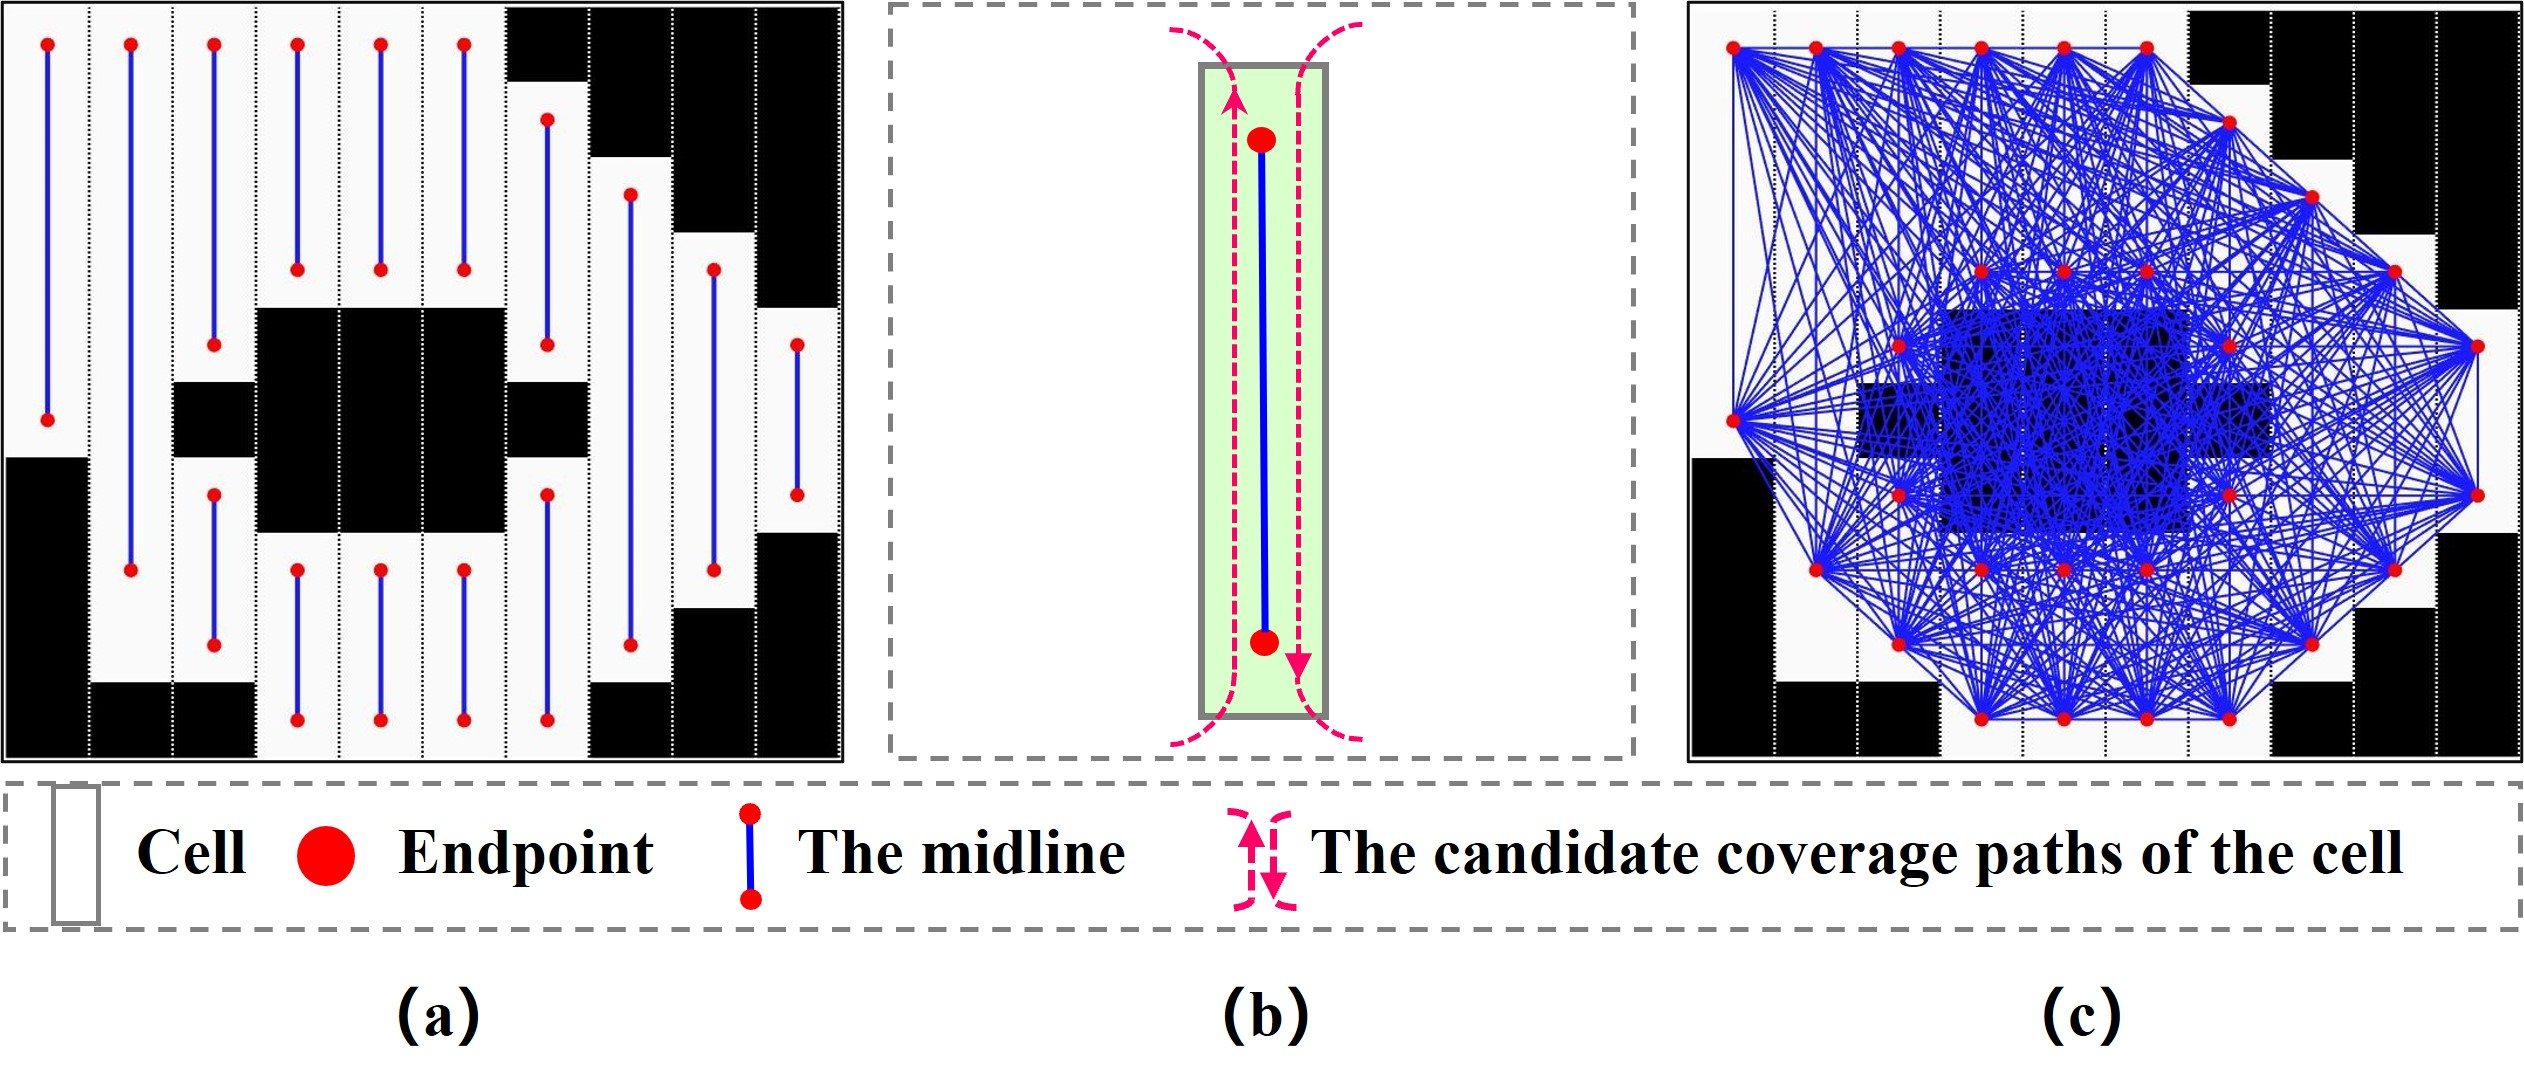
\includegraphics[width=0.8\textwidth]{2.jpg}
    \caption{ Graph representation. (a) Endpoints of each cell. (b) Coverage paths of each cell. (c) Graph.}
 %   \vspace{-0.2 cm} %设置与下面正文的距离
   \label{Fig_graph_representation}
\end{figure}

The edge between $v_i$ and $v_j$ represents the Dubins path from the start pose $v_i:(x_i,y_i,\theta_i)$ to the target pose $v_j:(x_j,y_j,\theta_j)$. The x/y coordinates $(x_i,y_i)$ and $(x_j,y_j)$ are fixed, but the angle $\theta_i$ and $\theta_j$ depends on $v_i$ and $v_j$'s relative positions. There are two cases for $\theta_i$ and $\theta_j$. In the first case, $v_i$ and $v_j$ belong to the same cell. Suppose that $v_i$ is the lower endpoint of the cell. The robot enters the cell from $v_i$ and covers the entire cell from bottom to top. Thus, $\theta_i$ and $\theta_j$ are set as $ \frac{\pi}{2} $; alternatively, $\theta_i = \theta_j = \frac{3\pi}{2}$. The second case is that $v_i$ and $v_j$ belong to different cells. $\theta_i$ will be set to $ \frac{3\pi}{2} $ if $v_i$ is the lower endpoint of the cell (i.e., the robot leaves the cell from its lower endpoint); otherwise, $\theta_i = \frac{\pi}{2}$. Similarly, $\theta_j$ will set $ \frac{\pi}{2} $ if $v_j$ is the lower endpoint of the cell (i.e., the robot enters the cell from its lower endpoint); otherwise, $\theta_j = \frac{3\pi}{2}$. Fig.\ref{Fig_pose} shows an example of how to calculate the angle. After determining the start and target pose, the Dubins path between $v_i$ and $v_j$ is calculated. The length of the Dubins path is set as the weight of $e_{i,j}$.

\begin{figure}[htb] %这里使用的是强制位置,除非真的放不下,不然就是写在哪里图就放在哪里,不会乱动
	\centering  %图片全局居中
    \vspace{0 cm} %设置与上面正文的距离
    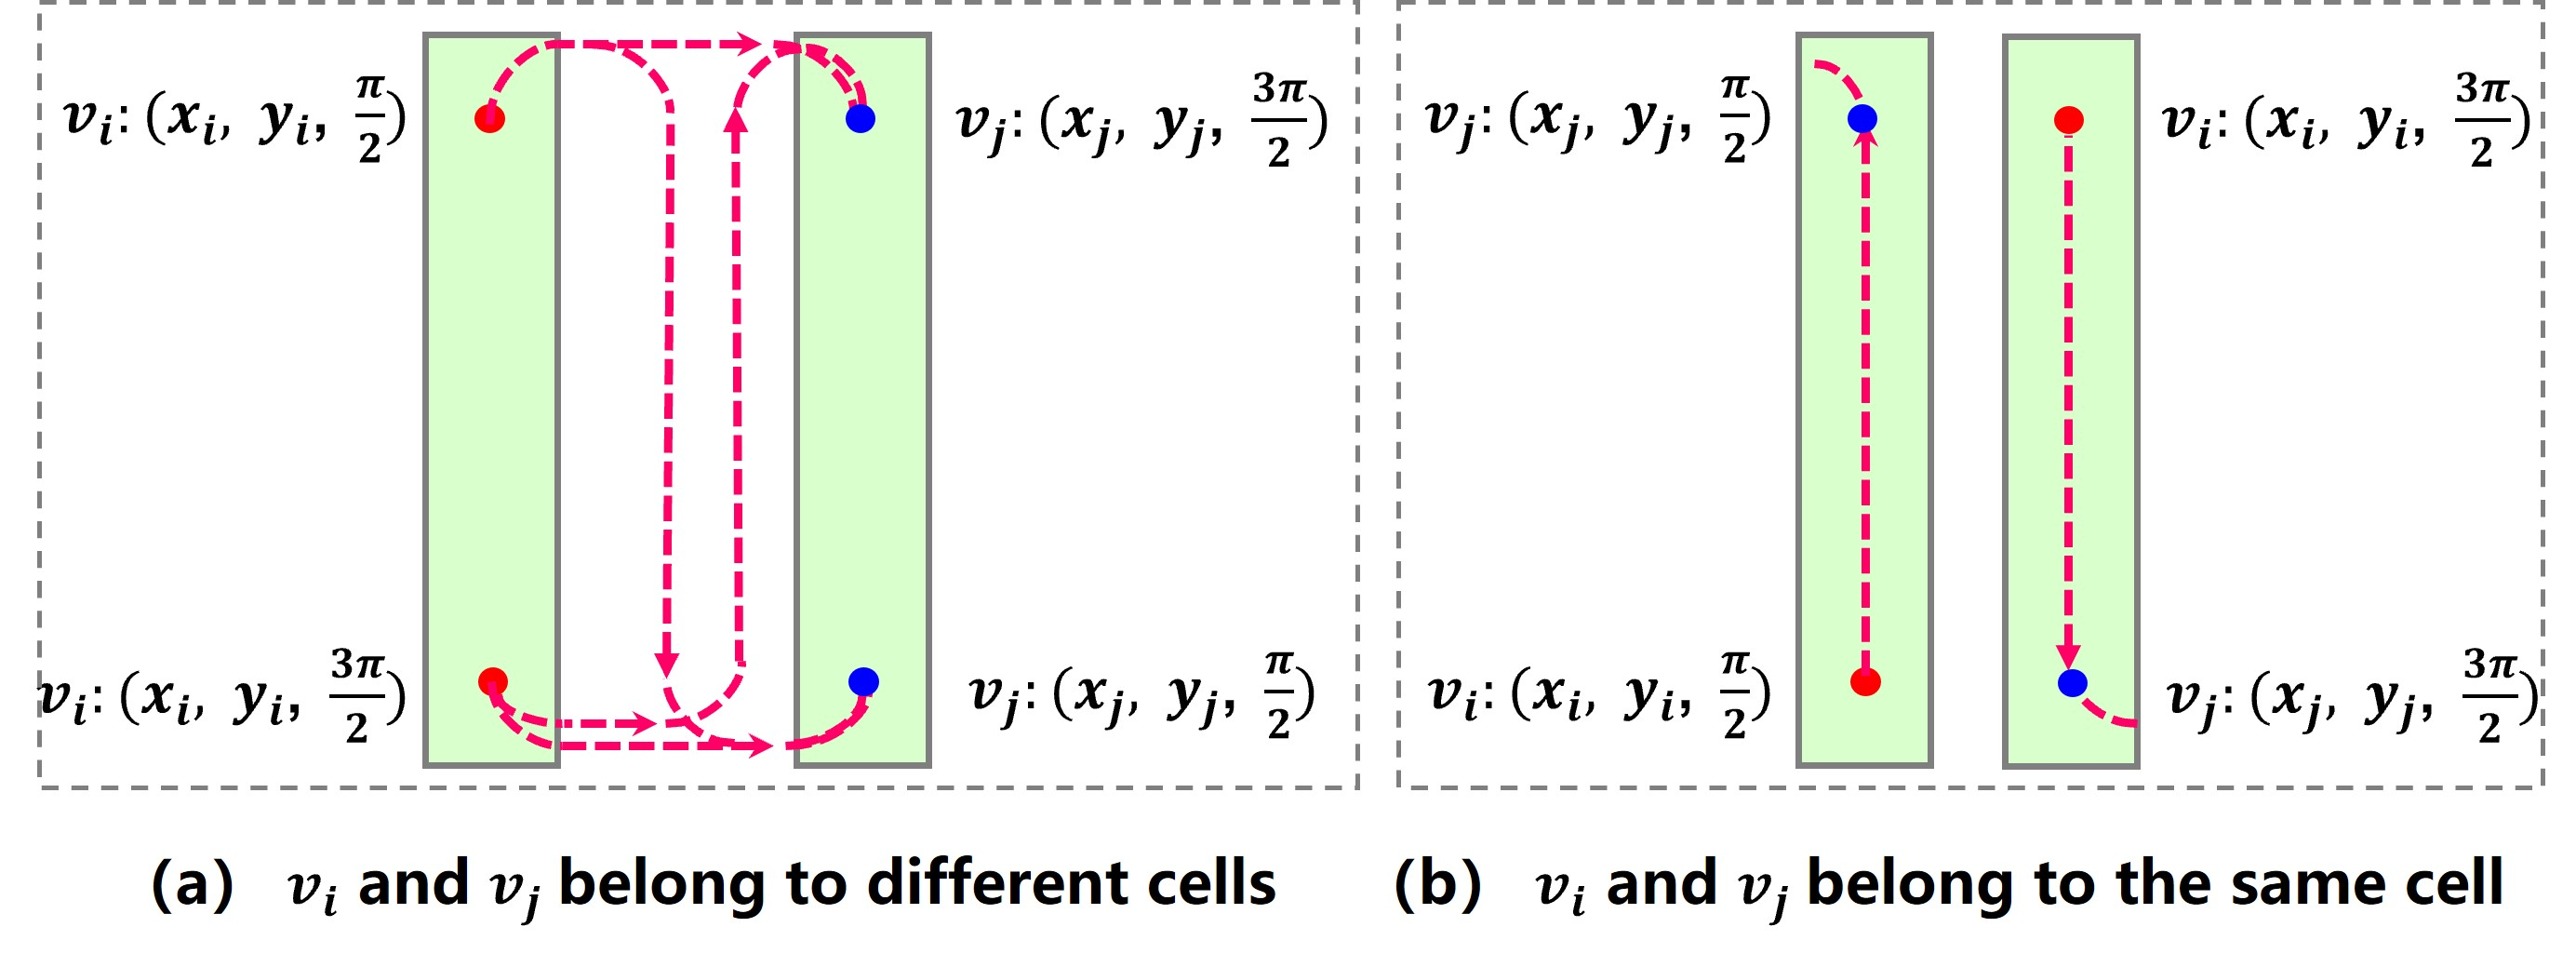
\includegraphics[width=0.9\textwidth]{3.jpg}
    \caption{ The start pose $v_i:(x_i,y_i,\theta_i)$ and target pose $v_j:(x_j,y_j,\theta_j)$.}
%    \vspace{-0.4 cm} %设置与下面正文的距离
   \label{Fig_pose}
\end{figure}

\subsection{Build MILP}

The optimal coverage aims to find $K$ tours that start and end at the depot $p_s$, so every point of allowed areas is visited, and the maximum cost of $K$ tours is minimized. Thus, \replaced{EDM}{EMD} models the Dubins MCPP problem as a MILP with the $MinMax$ objective of minimizing the longest path cost among $K$ robot paths. Define $t$ as the cost of the longest Dubins path. The objective is

\begin{equation}\label{Eq.objective}
\begin{aligned}
min(t)
\end{aligned}
\end{equation}
s.t.,
\begin{equation}\label{Eq.c2}
\begin{aligned}
t \geq \sum_{j=0}^{2N+1}\sum_{i=0}^{2N+1} x_{i,j,k}|e_{i,j}|, k=1,...,K
\end{aligned}
\end{equation}

\begin{equation}\label{Eq.c3}
\begin{aligned}
\sum_{k=1}^{K} y_{i,k} = 1, i=1,..,2N
\end{aligned}
\end{equation}

\begin{equation}\label{Eq.c4}
\begin{aligned}
\sum_{j=1}^{2N} x_{i,j,k} = y_{i,k}, i=1,..,2N, i \neq j, k=1,...,K
\end{aligned}
\end{equation}

\begin{equation}\label{Eq.c5}
\begin{aligned}
\sum_{j=1}^{2N} x_{j,i,k} = y_{i,k}, i=1,..,2N, i \neq j, k=1,...,K
\end{aligned}
\end{equation}


\begin{equation}\label{Eq.c6}
\begin{aligned}
% \left { x_{2i+1,2i+2,k} + x_{2i+2,2i+1,k} = y_{i,k},} \right. \\
%  \left. { i= 0,..,N-1, i \neq j, k=1,...,K} \right \\
%  x_{2i+1,2i+2,k} + x_{2i+2,2i+1,k} = y_{i,k}, i= 0,..,N-1, k= 1,...,K
\begin{split}
   x_{2i+1,2i+2,k} & + x_{2i+2,2i+1,k} = y_{i,k} \\
     & i= 0,..,N-1, k= 1,...,K
\end{split}
\end{aligned}
\end{equation}


\begin{equation}\label{Eq.c7}
\begin{aligned}
%u_{i,k} - u_{j,k} + Mx_{i,j,k} \leq M-1 i,j =1,..,2N, i \neq j, k=1,...,K
\begin{split}
   u_{i,k} &- u_{j,k} + Mx_{i,j,k} \leq M-1 \\
     &i,j =1,..,2N, i \neq j, k=1,...,K
\end{split}
\end{aligned}
\end{equation}

\begin{equation}\label{Eq.c8}
\begin{aligned}
x_{i,j,k} \in \{0,1\}, y_{i,k} \in \{0,1\}, \forall i,j,k
\end{aligned}
\end{equation}
where $x_{i,j,k} = 1$ represents that the robot $r_k$ visits vertex $j$ immediately after vertex $i$; otherwise, $x_{i,j,k} = 0$. $y_{i,k} = 1$ indicates that the robot $r_k$ visits vertex $i$; otherwise, $y_{i,k} = 0$. Eq.(\ref{Eq.c3}) states that each vertex should be visited exactly once. Eq.(\ref{Eq.c4})-(\ref{Eq.c5}) ensures that once a robot visits a vertex, it must also depart from the same vertex. Eq.(\ref{Eq.c6}) ensures that two endpoints of a cell should be traversed by sequence. Eq.(\ref{Eq.c7}) is the MTZ-based subtour elimination constraints \cite{miller1960integer}. The MILP is an extension of asymmetry multiple traveling salesman problems (MTSP).


\subsection{Pseudo-code of the \replaced{EDM}{EMD} algorithm}
Algorithm \ref{alg:EMD Algorithm} shows the pseudo-code of the \replaced{EDM}{EMD} algorithm. It inputs the region ($\cal{A}$), the robot set ($R$) and starting point ($p_s$) and outputs $K$ coverage paths $\{P_1, ...,P_K\}$. First, $K$ coverage paths are initialized as empty (Line 1), and the region $\cal{A}$ has been divided into a set of cells $C$ (Line 2). The cell set $C$ is represented as a graph $G$ (Line 3), and the cost matrix associated with $G$ is calculated (Line 4). \replaced{EDM}{EMD} models the Dubins MCPP problem as a MILP (Line 5) and utilizes the MILP Solver \cite{bixby2007gurobi}  to obtain the traversal sequence $\{T_1, ..., T_K\}$ (Line 6). Coverage paths are calculated according to $\{T_1, ...,T_K\}$ (Line 7).

\begin{algorithm}[htbp]
  \caption{EDM Algorithm}
  \label{alg:EMD Algorithm}
\textbf{Input}:  $ \cal{A}, R$, $p_s$\\
%\textbf{Parameter}: Optional list of parameters\\
\textbf{Output}: $P_1, ...,P_K$
\begin{algorithmic}[1] %[1] enables line numbers
\STATE Initialize: $P_1, ...,P_K \gets \emptyset$;
\STATE $C \gets$ Area\_Decomposition($ \cal{A}$);
\STATE $G \gets$ Graph\_Representation($C, p_s$);
\STATE $CostMatrix \gets$ calculate the cost between points in $G$
\STATE Build\_MILP($G$); // Eq.(1) - Eq.(7)
\STATE $\{T_1, ...,T_K\} \gets$  MILP\_Solver;
\STATE $\{P_1, ...,P_K\} \gets$  Dubins\_Solver($\{V_1,...,V_K\}$);
\STATE \textbf{return} $P_1, ...,P_K$
\end{algorithmic}
\end{algorithm}


\textit{Computational Complexity}: Let $M$ be the number of vertexes in $G$. The cost matrix can be calculated in $\cal{O}$$(M^2)$ times. The asymmetry MTSP can be transformed into an asymmetry TSP, which tasks $\cal{O}$$(M^3)$ times in the worst case \cite{frieze1982worst}. Thus, the overall complexity of \replaced{EDM}{EMD} is $\cal{O}$$(M^{3})$.


\section{ Heuristic Credit-based \replaced{Dubin Multi-robot CPP(CDM)}{Multi-robot Dubin CPP (CMD)} Algorithm}
\label{Sec_CMD}
\replaced{EDM}{EMD} algorithm provides an effective weapon to plan exact coverage paths for small-scale coverage applications. However, several coverage applications involve a large number of coverage tasks and allow for near-optimal results. Therefore, this paper presents a heuristic \replaced{CDM}{CMD} algorithm consisting of three components: initial partition, partition refinement, and path planning. The initial partition component utilizes the regional growth strategy to divide the region into $K$ subareas. The partition refinement component balances $K$ subareas by a tree-partition strategy, and the path planning component employs the single-robot Dubins solver \cite{c25} to each subarea.

%However, it suffers from three limitations. First, the credit-based coverage method can only perform coverage applications based on grid decomposition, and is not applicable to other coverage applications such as Morse decomposition or Semi-BCD decomposition. Secondly, CTA algorithm assumes that $K$ robots Randomly locates at different starting points in the target region. However, randomly initializing the locations of robots is less practical because it forces robots to divert time and resources to localization and movement to the desired starting location. Finally, CTA algorithm does not consider the kinematic constraints of the robot.

\subsection{Initial Partition}

As mentioned in \ref{subsec_Problem_Statement}, the mission environment has been divided into a set of cells $C$. The initial partition component represents $C$ as a connected graph $G1 = \{V1,E1\}$, where the vertex represents the cell, and the edge represents the common border between cells. Fig.\ref{Fig_4} shows an example of the graph representation. The region growth strategy based on the credit model \cite{li2022complete} is used to divide the region (i.e., the graph $G1$) into $K$ partitions.

\begin{figure}[htb] %这里使用的是强制位置,除非真的放不下,不然就是写在哪里图就放在哪里,不会乱动
	\centering  %图片全局居中
    \vspace{0 cm} %设置与上面正文的距离
    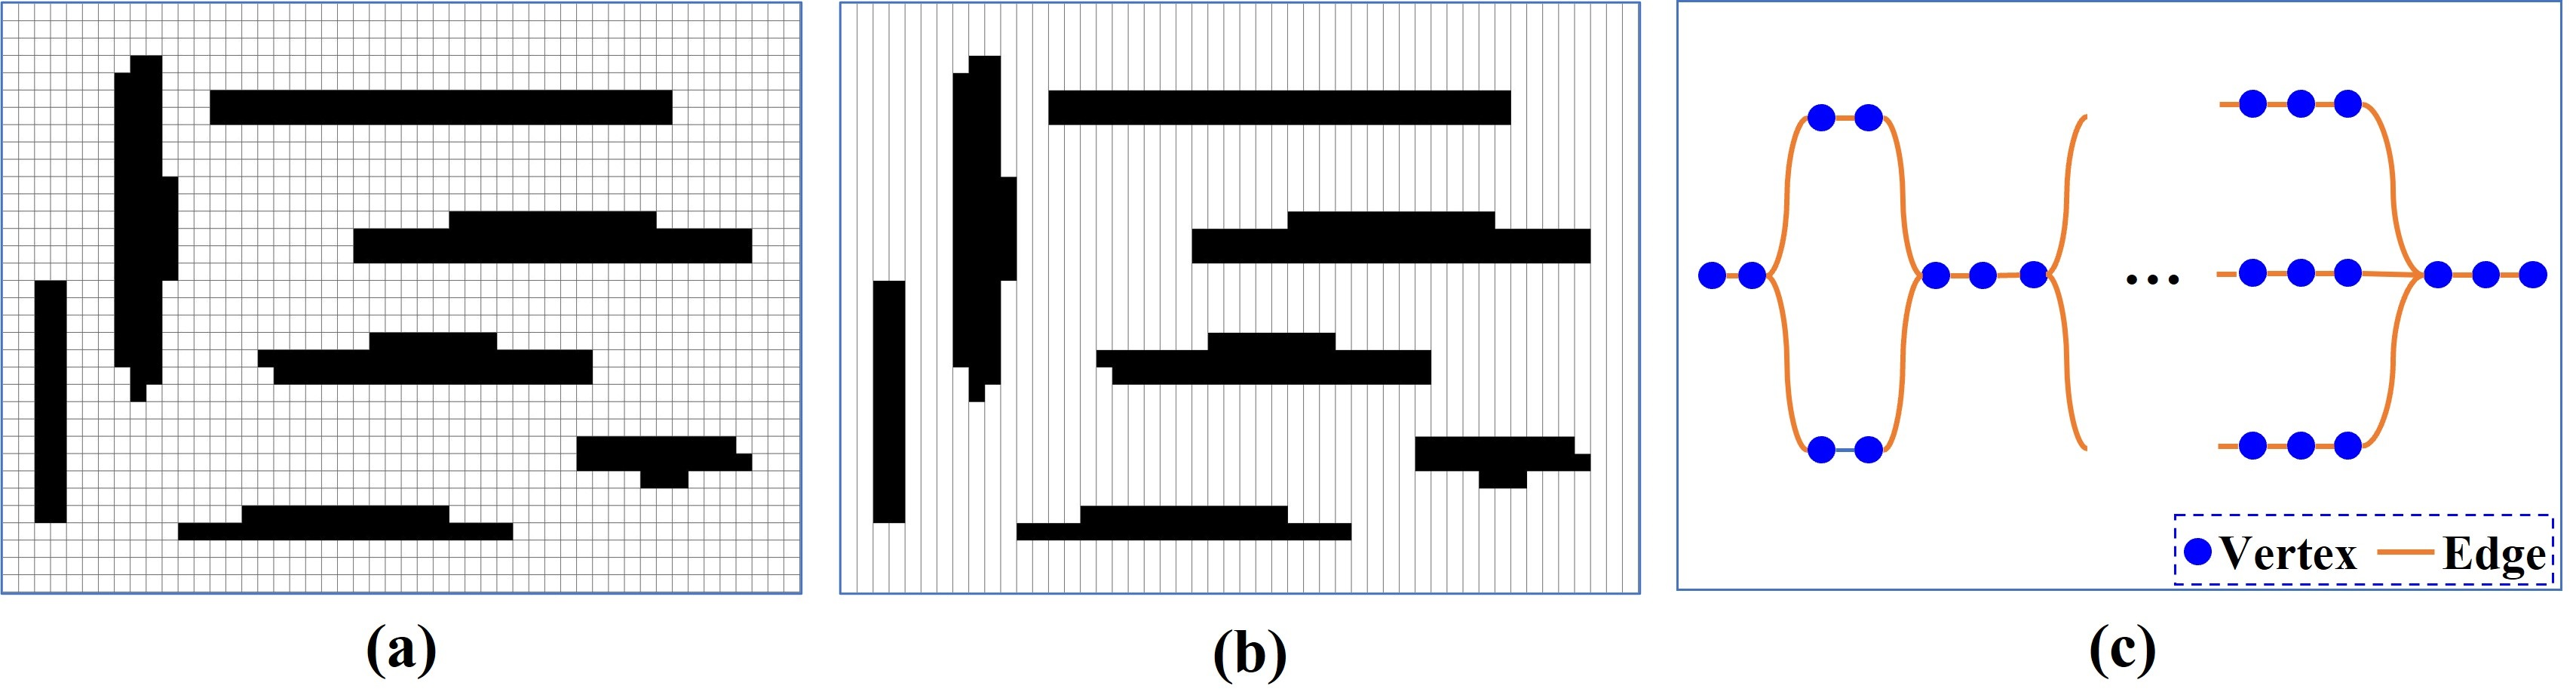
\includegraphics[width=0.9\textwidth]{4.jpg}
    \caption{ Graph representation. (a) The input map. (b) Coverage cells. (c) The connected graph.}
    %\vspace{-0.4 cm} %设置与下面正文的距离
   \label{Fig_4}
\end{figure}

In the credit model, $K$ partitions act as traders in the virtual economy. Coverage cells are tradable commodities with measurable values. Additionally, a virtual bank is introduced. Traders can open credit accounts with a balance equal to $\frac{w(V1)}{K}$. The virtual bank maintains accounts and manages assets for traders. Each trader can borrow from the bank (without interest) if his account balance reaches zero. When a trader buys a cell $v_t$, its account balance is reduced by $|v_t|$, where $|v_t|$ represents the area of the cell $v_t$. On the other hand, if a trader sells a cell $v_t$, the account balance increases by $|v_t|$. Traders continue to buy cells, and the corresponding account balance decreases.

\begin{figure}[htb] %这里使用的是强制位置,除非真的放不下,不然就是写在哪里图就放在哪里,不会乱动
	\centering  %图片全局居中
    \vspace{0 cm} %设置与上面正文的距离
    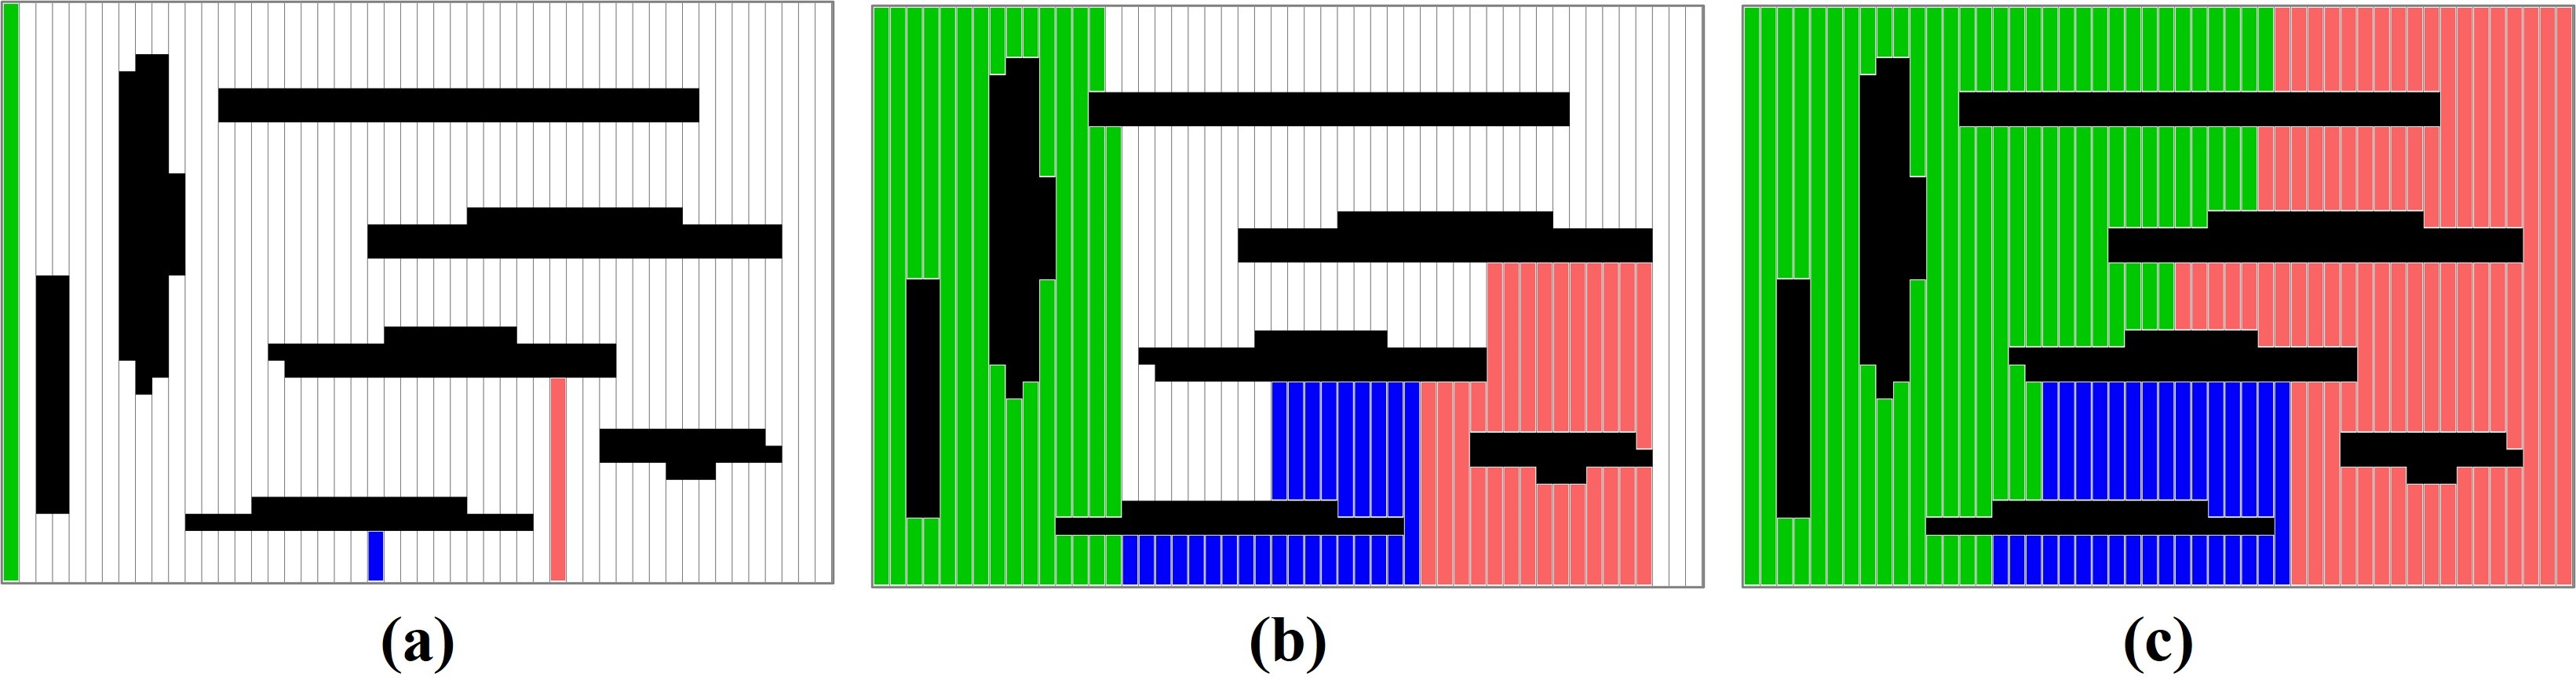
\includegraphics[width=0.8\textwidth]{5.jpg}
    \caption{An example of the initial partition for three robots.}
    %\vspace{-0.4 cm} %设置与下面正文的距离
   \label{Fig_5}
\end{figure}

The initial partition component uses the regional growth strategy to divide the region into $K$ partitions. First, cells in $C$ are sorted in increasing order by the x-coordinate, followed by the y-coordinate, resulting in a sequence of cells $S$. The $K$ cells, distributed at equal intervals in $S$, are set as the seeds of the K partitions. Second, every partition alternately buys cells and grows around the seed as the number of bought cells increases. All partitions become larger and larger until all cells in $G1$ have been purchased. In this case, $G1$ has been divided into $K$ partitions. Fig.\ref{Fig_5} shows an example of the region growth strategy.

\subsection{Partition Refinement}
Due to complex obstacles, the initial $K$ partitions may not be balanced. In order to obtain a balanced result, the partition refinement component reallocates tasks among partitions by way of task transactions. Each task transaction is performed in three steps. The first step is to determine the two partitions for the task transaction. The $k$-th partition (i.e., $V_k$) with the largest account balance is set as the buyer, i.e., the partition that receives tasks. Let $ADV$ be the set of partitions adjacent to $V_k$. The partition $u \in ADV$ that has the greatest difference with the account balance of $V_k$ becomes the seller, i.e., the partition that dispatchs tasks.
$found(k)$ and $found(u)$ represents the account balance of the seller and buyer, respectively.
% Let $found'(k)$ and $found'(u)$ be the account balance of the seller and buyer before the task transaction.

\begin{figure}[htbb] %这里使用的是强制位置,除非真的放不下,不然就是写在哪里图就放在哪里,不会乱动
	\centering  %图片全局居中
    \vspace{0 cm} %设置与上面正文的距离
    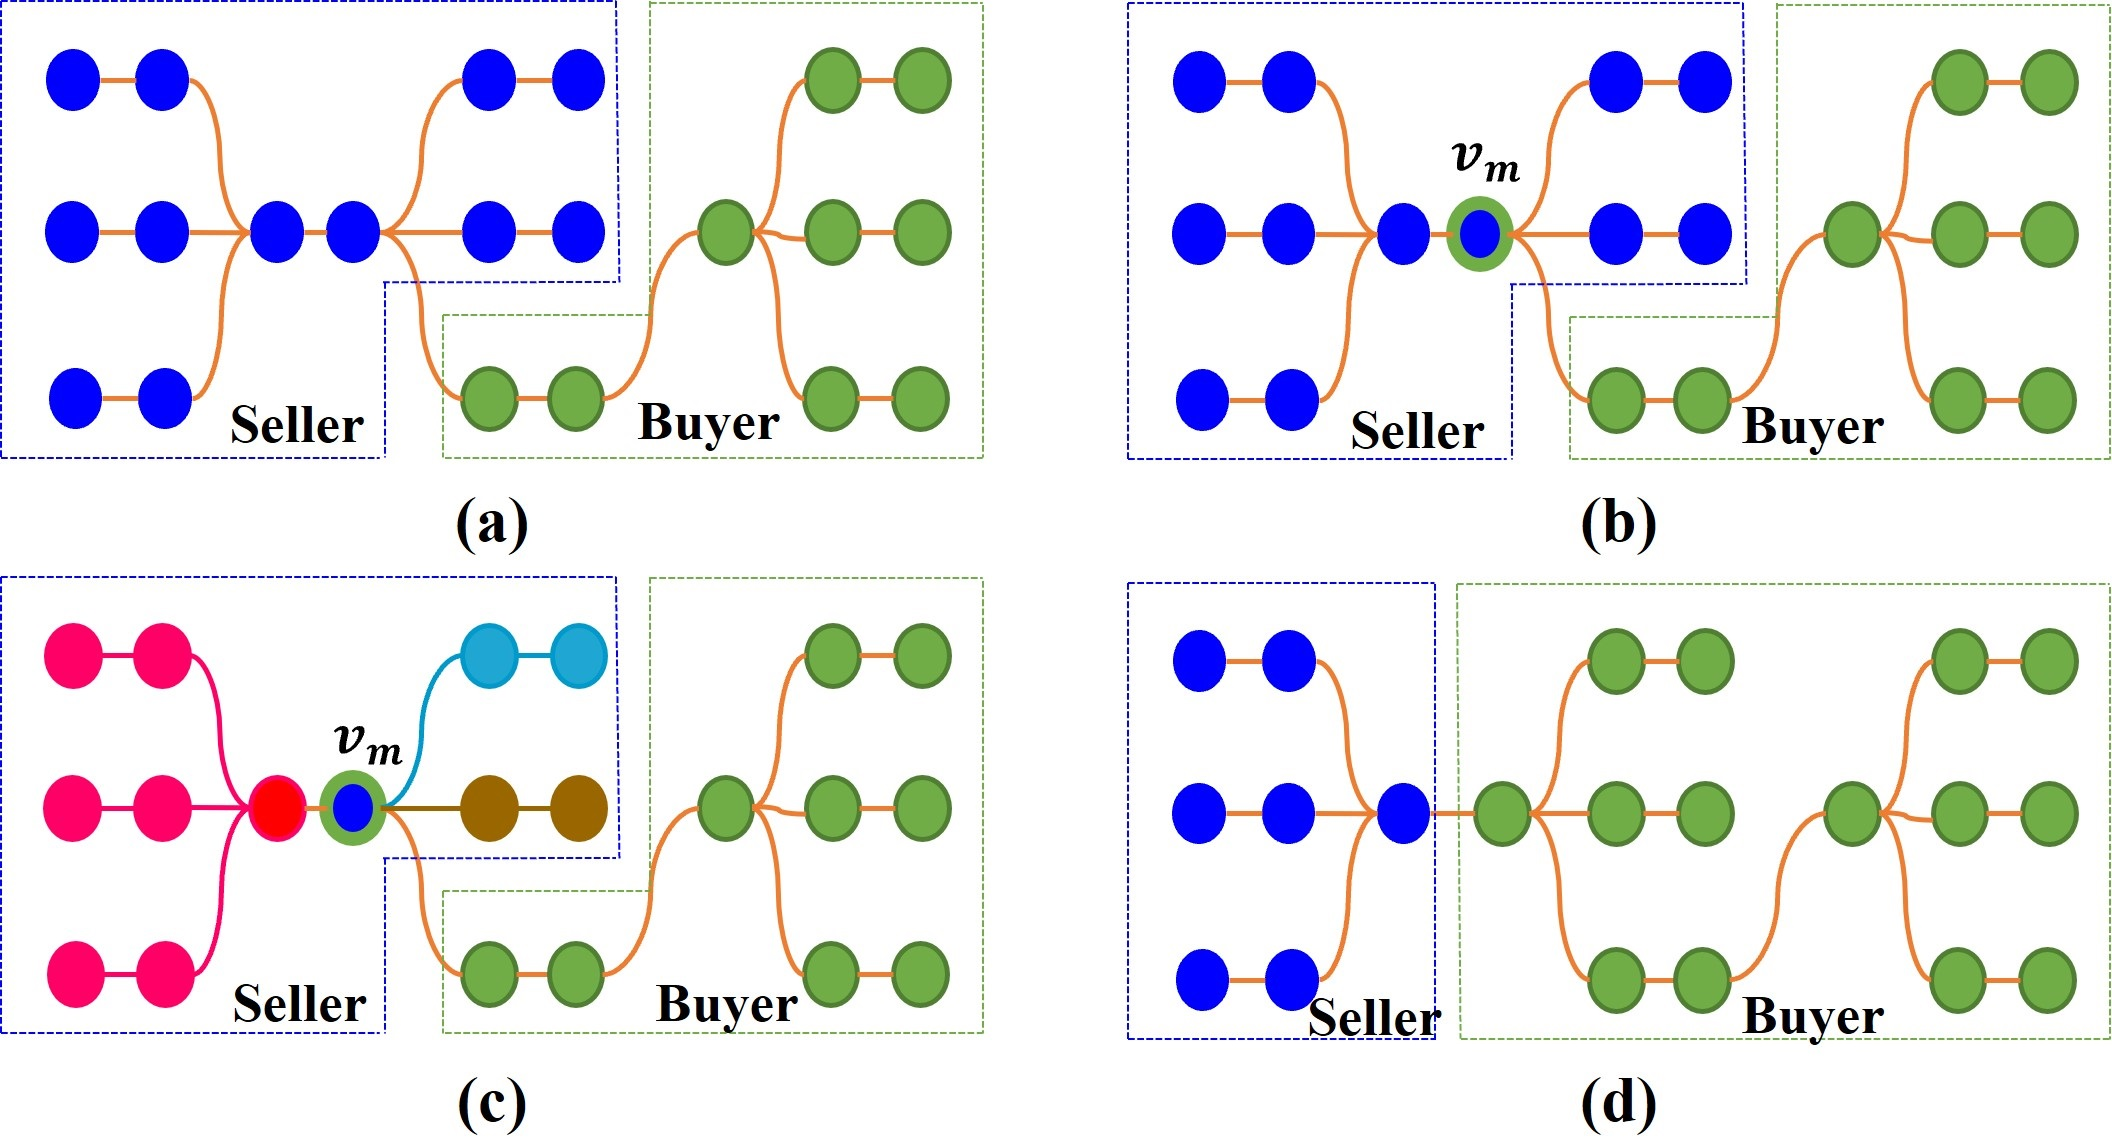
\includegraphics[width=0.75\textwidth]{6.jpg}
    \caption{ An example of the tree-partition strategy. (a) The graphs of the seller and buyer. (b) The adjacent vertex $v_m$. (c) Three subtrees with the root $v_m$ in the seller. (d) The buyer and seller after the task transcation.}
    %\vspace{-0.2 cm} %设置与下面正文的距离
   \label{Fig_6}
\end{figure}

The second step is to decide which tasks the seller and buyer will trade. Suppose that $AC \in V_u$ is the cell set that shares a common border with $V_k$. The cell $v_m$ with the biggest weight in $AC$ is selected for the candidate trade task $EV$. There are two possible cases, depending on the connection between $v_m$ and $V_u$. In the first case, $v_m$ is not the cut point of $V_u$. The trade task $EV$ is set as $v_m$ since both seller and buyer remain connected after the task transaction. The second case is that $v_m$ is the cut point of $V_u$ (i.e., removing $v_m$ disconnects $V_u$). The seller $V_u$ becomes disconnected if it sells $v_m$ to $V_k$. However, disconnect partitions cause robot collisions and complicate robot control \cite{c1}. Thus, the depth first search (DFS) method is utilized to find the $Q$ subtrees $\{V_{u,1}, ...V_{u, Q}\}$ in $V_u$ whose root nodes are $v_m$. $V_{u,i}$ and $V_{u,j}, i \neq j, i,j=1,...,Q$ will be disconnected if $v_m$ is removed from $V_u$. In order to maintain its connectivity, the seller $V_u$ needs to reserve one subtree and set the other tasks as trade tasks. In order to determine which subtree the seller retains, a transaction index is defined, which quantifies the balance between the buyer and seller's tasks. Suppose the seller reserves the $q$-th subtree $V_{u,q}$. The seller and the buyer will be updated to $V_{k'} = V_k \cup (V_u - V_{u,q})$ and $V_{u'} = V_{u,q}$, respectively. The trade index $\delta_q$ of the $q$-th subtree is set as $max(abs(found(k'),found(u')))$, where $found(k')$ and $found(u')$ represents the account balance of $V_{k'}$ and $V_{u'}$. $Q$ subtrees correspond to $Q$ trade indexes $\{\delta_1,...,\delta_Q\}$. The smaller the trade index, the more balanced the buyer and seller. Let $\delta_{q1}$ be the minimum of $\{\delta_1,...,\delta_Q\}$, and $\delta_B$ be the trade index of $V_k$ and $V_u$. If $\delta_{q1} < \delta_B$, the seller retains the $V_{u,q1}$ with the least transaction index. The remaining tasks $V_u - V_{u,q1}$ are set as the trade tasks, i.e., $EV = V_u - V_{u,q1}$. Fig.\replaced{\ref{Fig_6}}{\ref{Eq.c6}}shows an example of the tree-partition strategy. Alternatively, $\delta_{q1} > \delta_B$ indicates that the tasks of the seller and the buyer do not become balanced after the task transaction. A new $v_m$ from $AC$ is set as the candidate trade task $EV$, and the tree-partition strategy is applied for the new $v_m$. If all cells in $AC$ can not provide more balance partitions, a new task transaction is performed since $V_u$ and $V_k$ are a pair of non-tradable partitions. With the tree-partition strategy, a set of tasks rather than a single task are reallocated, while keeping the connectivity of partitions.

In the third step, the buyer and seller trade tasks and update their account balances. The buyer $V_k$ purchases the task set $EV$, and its account balance becomes $w(V_k)-w(EV)+D_{s,k}$, where $w(EV)$ and $D_{s,k}$ represent the sum of weights of $EV$ and the shortest distance between the starting point $p_s$ and $V_k$. $D_{s,k}$ is calculated so the farther-distance traveling robot is compensated by assigning fewer tasks instead of dividing the region into $K$ equal sections. Similarly, the seller $V_u$ sells the task set $EV$ and adjusts its account balance to $w(V_u)+w(EV)+D_{s,u}$, where $D_{s,u}$ represents the shortest distance between the starting point $p_s$ and $V_u$.

With the completion of task transactions, the $K$ partitions become more and more balanced. As soon as the number of task transactions reaches the preset upper limit, the partition refinement component ends and returns $K$ partitions $\{V_1,..., V_K\}$.


\subsection{Path Planning}

After receiving $K$ partitions from the partition refinement component, the path planning component applies the single-robot Dubins solver \cite{c56} to each partition. A set of $K$ Dubins coverage paths is generated, and each one corresponding to one robot. The complete coverage is achieved if each robot moves along the corresponding coverage path. Fig.\replaced{\ref{Fig_7}}{\ref{Eq.c7}} shows an example of the \replaced{CDM}{CMD} algorithm.

\begin{figure}[htb] %这里使用的是强制位置,除非真的放不下,不然就是写在哪里图就放在哪里,不会乱动
	\centering  %图片全局居中
    \vspace{0 cm} %设置与上面正文的距离
    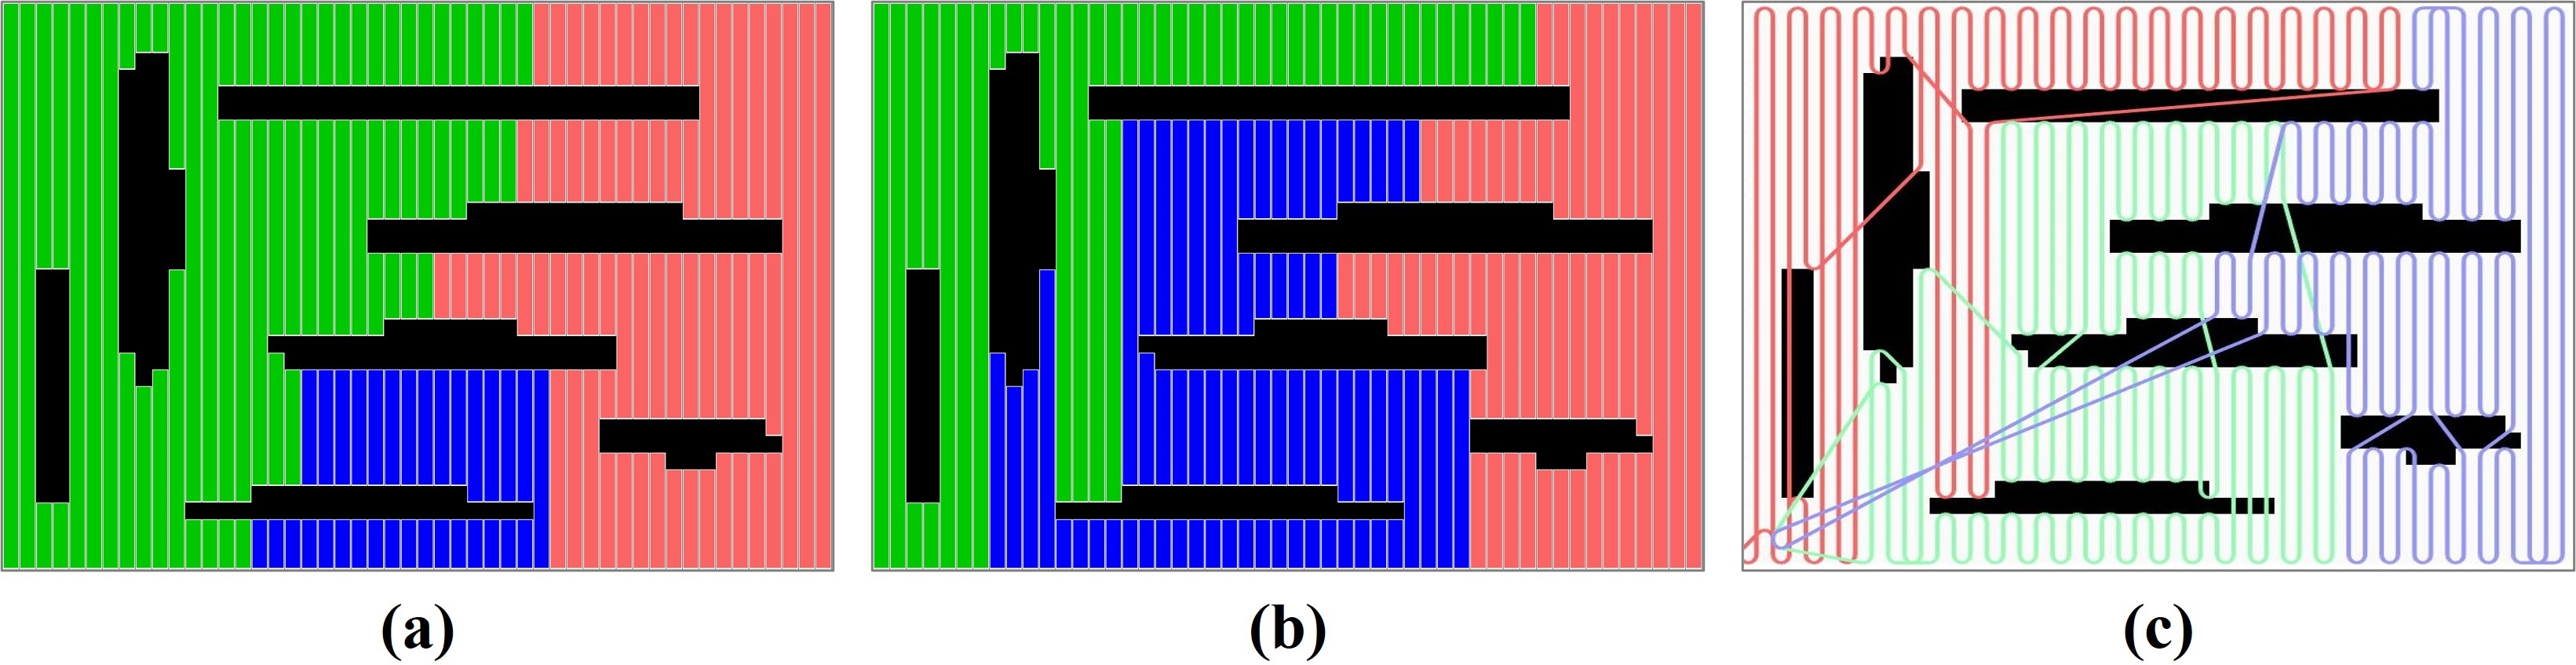
\includegraphics[width=0.8\textwidth]{7.jpg}
    \caption{ (a) Initial partition. (b) Partition refinement. (c) Path Planning.}
    \vspace{-0.2 cm} %设置与下面正文的距离
   \label{Fig_7}
\end{figure}


\subsection{Pseudo-code of the \replaced{CDM}{CMD} algorithm}

Algorithm \ref{alg:CMD Algorithm} shows the pseudo-code of the \replaced{CDM}{CMD} algorithm. It decomposes the region $\cal{A}$ into a set of cells $C$ and represents all cells into a graph $G1$ (Lines 2-3). The graph $G$ is divided into $K$ partitions by the initial partition (Line 4). These $K$ partitions are refined by task transactions (Lines 5-23). For each task transaction, the buyer $V_k$ and the seller $V_u$ are determined, followed by the set of adjacent cells $AC$ between $V_k$ and $V_u$ (Lines 7-8). The seller $V_u$ is the partition that is adjacent to and can trade with $V_k$. For each cell in $AC$, the tree-partition strategy calculates the corresponding trade tasks $EV$ (Line 11). If $EV \neq \emptyset$, $V_k$ and $V_u$ trade tasks and updates their account balances (Lines 13-14). The symbol $succeed$, which indicates the success of the task transaction, is marked as $true$ (Line 15). If $succeed$ remains $false$, $V_k$ and $V_u$ are marked as a pair of non-tradable partitions (Lines 19-21). Upon the number of task transactions equaling $MaxI$, $K$ partitions $\{P_1, ...,P_K\}$ is obtained. Next, the single-robot Dubins solver \cite{c25} is used for each partition to generate coverage paths $\{P_1, ...,P_K\}$ (Lines 24).


\begin{algorithm}[hb]
\caption{CDM Algorithm}
\label{alg:CMD Algorithm}
\textbf{Input}: $ \cal{A}, R$, $p_s $\\
\textbf{Parameter}: $MaxI$: The maximum number of task transactions\\
\textbf{Output}: $P_1, ...,P_K$
\begin{algorithmic}[1] %[1] enables line numbers
\STATE Initialize: $P_1, ...,P_K \gets \emptyset$;
\STATE $C \gets$ Area\_Decomposition($ \cal{A}$);
\STATE $G1 \gets$ Graph\_Representation($C, p_s$);
\STATE $found, V_1,...,V_K \gets$ initial\_partition($G1, s$);
\STATE $count \gets 0$;
\WHILE{$count < MaxI$ }
    \STATE $V_k, V_u \gets$ determine the seller and the buyer;
    \STATE $AC \gets$ calculate the set of adjacent cells between $V_k$ and $V_u$;
    \STATE $succeed \gets false$;
    \FOR{each $v_m$ in $AC$}
        \STATE $EV \gets$ tree\_partition($V_k,V_u,v_m$);
        \IF{$EV \neq \emptyset$}
            \STATE Trade tasks $EV$;
            \STATE Update $found$;
            \STATE $succeed \gets true$;
            \STATE break;
        \ENDIF
    \ENDFOR

    \IF{$succeed = false$}
        \STATE Mark $V_k$ and $V_u$ as a pair of non-tradable partitions.
    \ENDIF

    \STATE $count ++$;
\ENDWHILE
\STATE $\{P_1, ...,P_K\} \gets$  Dubins\_Solver($\{V_1,...,V_K\}$);

\STATE \textbf{return} $P_1, ...,P_K$;
\end{algorithmic}
\end{algorithm}


\textit{Computational Complexity}: Let $M$ be the number of cells in $C$. The initial partition component takes $\cal{O}$$(M)$ times. The complexity of the partition refinement component is $\cal{O}$$(M*MaxI)$ in the worst case, but the worst cases are scarce. The Dubins solver takes $\cal{O}$$(M^3)$ times to calculate the Dubins path\cite{frieze1982worst}. Thus, the overall complexity of the \replaced{CDM}{CMD} algorithm is $\cal{O}$$(M^3)$.

\section{Experiments}
\label{Sec_Experiments}
The computational experiments were carried out on a PC with Intel(R) Core(TM) CPU i5-8300H, 2.30 GHz processor, 16G RAM, WIN 10. All experiments were performed on Dubins robots with kinematic constraints such as a forward speed of 1.0 m/s and a minimum turning radius of 1 m. A task sensor with a detection range of 1 m was incorporated into each robot. First, to demonstrate the superiority of the proposed algorithms, comparison experiments with exact and heuristic algorithms were conducted on different size maps. Second, simulation experiments based on a high-fidelity UAV model \cite{UAVsimulated} were conducted to verify the feasibility of \replaced{EDM}{EMD} and \replaced{CDM}{CMD}.

\subsection{Comparison experiments in small scenes}

The first level of validation was done via simulations on four small scenes with 10 m $\times$ 10 m $\times$ 10 m. Fig.\ref{Fig_8} demonstrates the point cloud maps of four scenes, which contain several obstacles with irregular shapes and same heights. For each scene, Dubins robots start and end at the same starting point, located in the bottom left corner of the map. \replaced{EDM}{EMD} and \replaced{CDM}{CMD} were compared with the exact Milpflow algorithm \cite{c39} and heuristic DCRC algorithm \cite{karapetyan2018multi}. Milpflow provides a precise area-division result instead of coverage paths. In order to achieve a fair comparison, the state-of-art Dubins solver \cite{c25} is employed to plan Dubins path for Milpflow. DCRC generates an optimal Hamiltonian path and divides the path into $K$ subpaths. Exact Mofint and \replaced{EDM}{EMD} algorithms utilize the Gurobi optimization tool \cite{bixby2007gurobi} to obtain the optimal solution, and their optimization time is uniformly set as 1200 s.


\begin{figure}[htbp] %这里使用的是强制位置,除非真的放不下,不然就是写在哪里图就放在哪里,不会乱动
	\centering  %图片全局居中
    \vspace{0 cm} %设置与上面正文的距离
    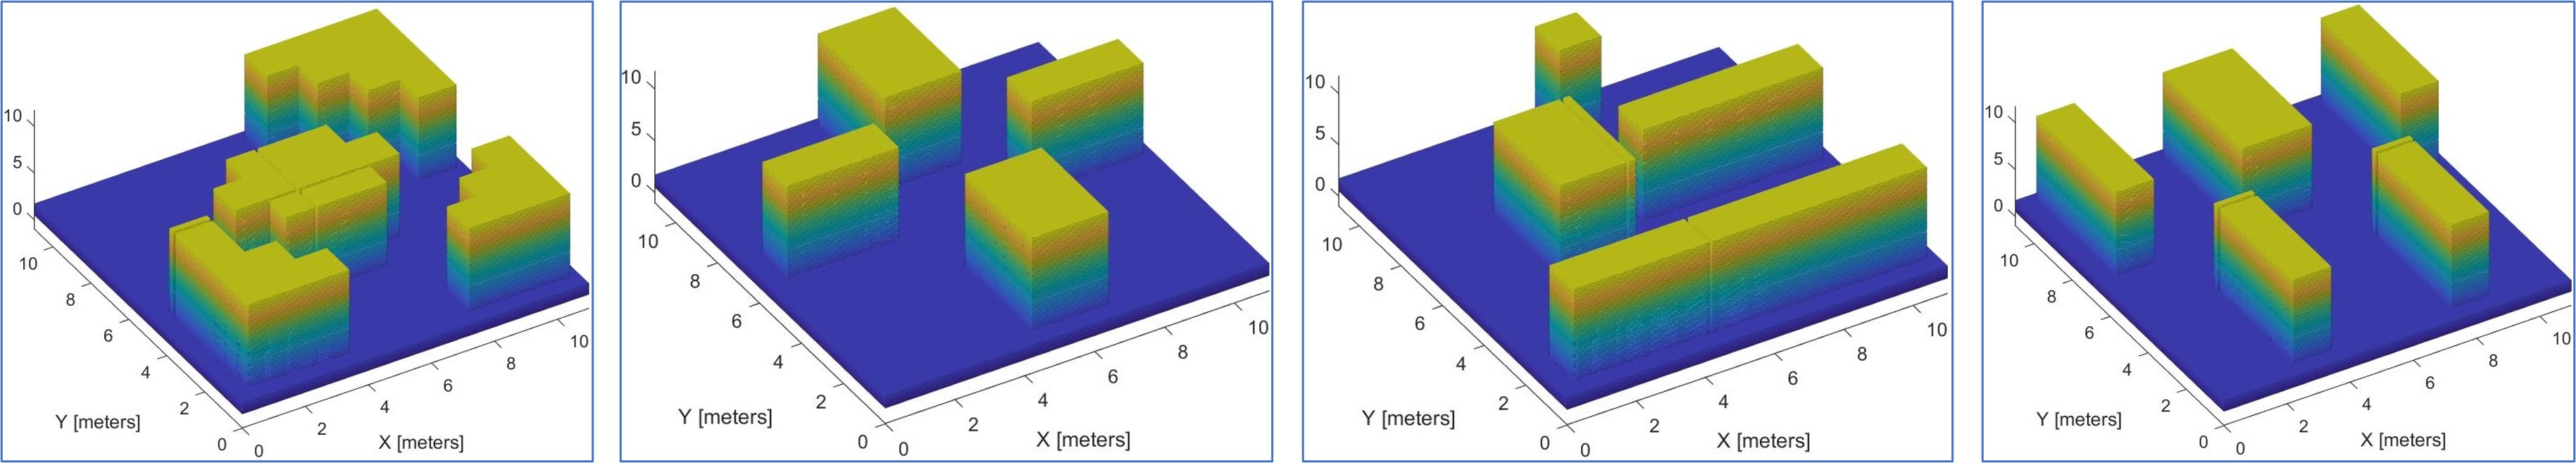
\includegraphics[width=0.98\textwidth]{8.jpg}
    \caption{ The four point-cloud maps where \replaced{EDM}{EMD} and \replaced{CDM}{CMD} were tested. Each environment is with the size of 10 m $\times$ 10 m $\times$ 10 m. }
    %\vspace{-0.4 cm} %设置与下面正文的距离
   \label{Fig_8}
\end{figure}



\begin{figure}[htbp] %这里使用的是强制位置,除非真的放不下,不然就是写在哪里图就放在哪里,不会乱动
	\centering  %图片全局居中
    \vspace{0 cm} %设置与上面正文的距离
    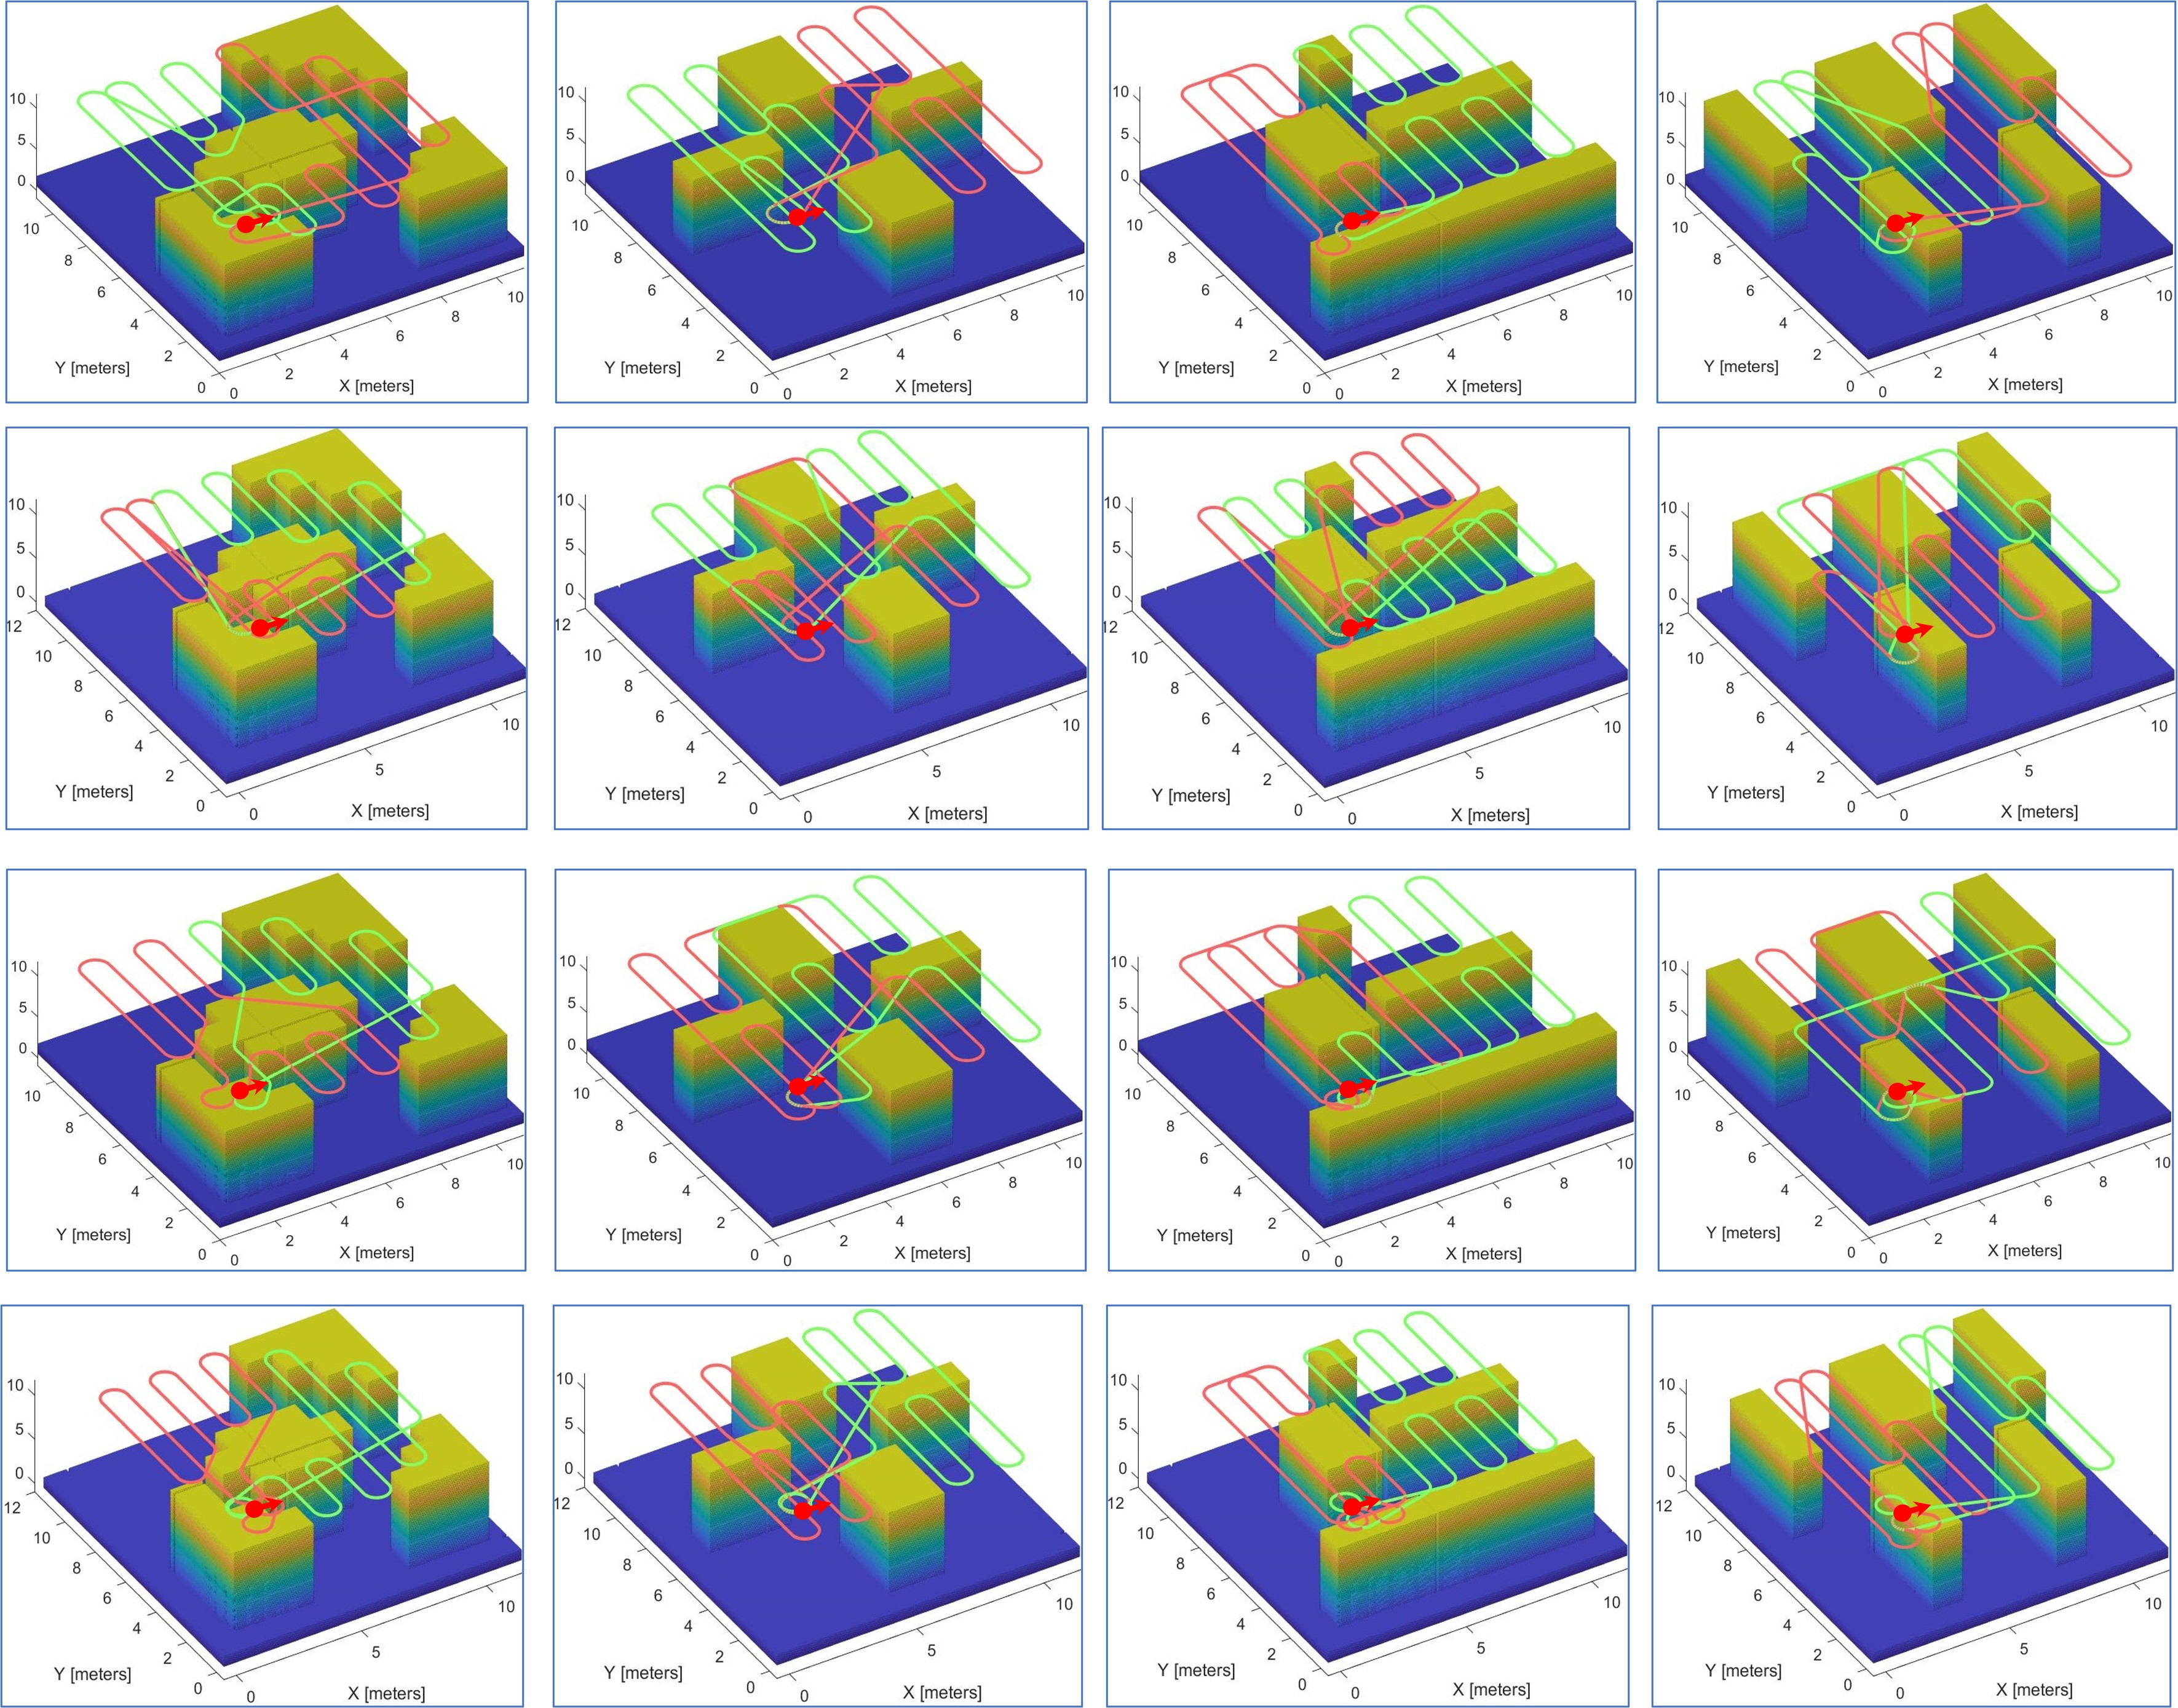
\includegraphics[width=0.92\textwidth]{8a.jpg}
    \caption{ Simulation instances with two robots. The first to fourth rows represent the snapshots of coverage paths provided by Milpflow \cite{c39}, DCRC \cite{karapetyan2018multi}, \replaced{EDM}{EMD}, and \replaced{CDM}{CMD}, respectively. }
    \vspace{-0.2 cm} %设置与下面正文的距离
   \label{Fig_8a}
\end{figure}


\begin{figure}[htbp] %这里使用的是强制位置,除非真的放不下,不然就是写在哪里图就放在哪里,不会乱动
	\centering  %图片全局居中
    \vspace{0 cm} %设置与上面正文的距离
    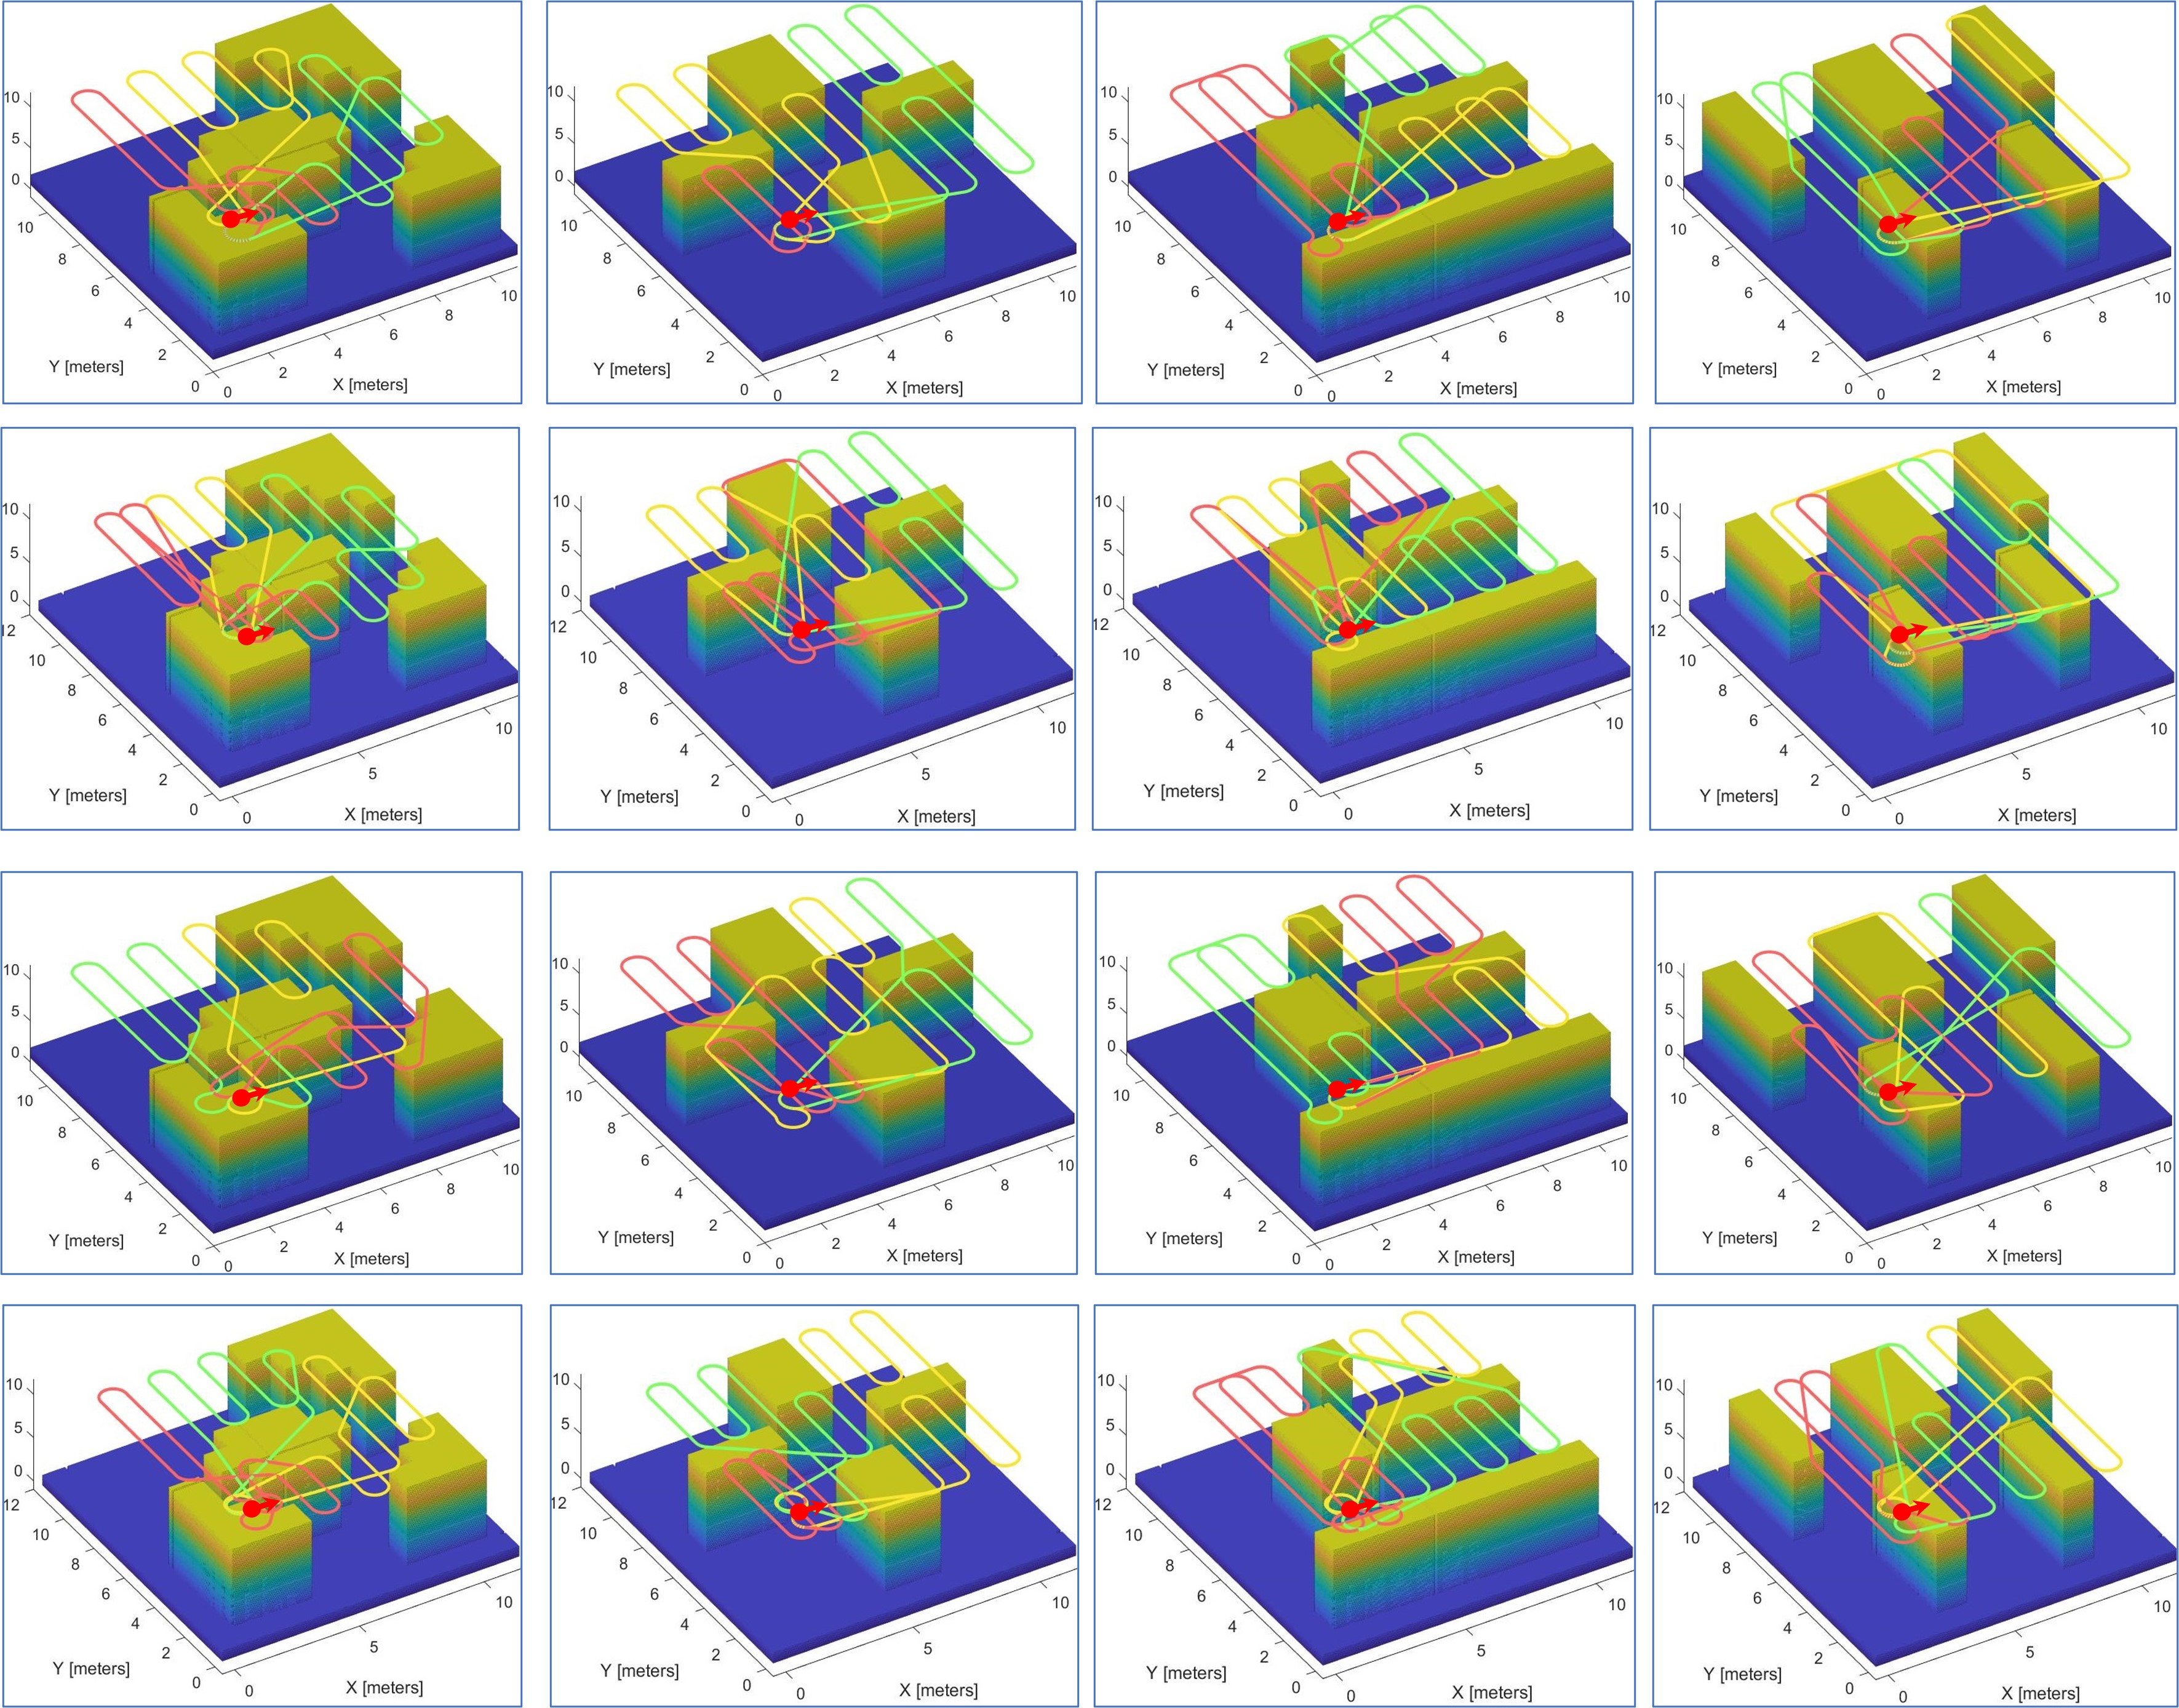
\includegraphics[width=0.92\textwidth]{8b.jpg}
    \caption{Simulation instances with three robots. The first to fourth rows represent the snapshots of coverage paths provided by Milpflow \cite{c39}, DCRC \cite{karapetyan2018multi}, \replaced{EDM}{EMD}, and \replaced{CDM}{CMD}, respectively.  }
    %\vspace{-0.4 cm} %设置与下面正文的距离
   \label{Fig_8b}
\end{figure}

\begin{figure}[htb] %这里使用的是强制位置,除非真的放不下,不然就是写在哪里图就放在哪里,不会乱动
	\centering  %图片全局居中
    \vspace{0 cm} %设置与上面正文的距离
    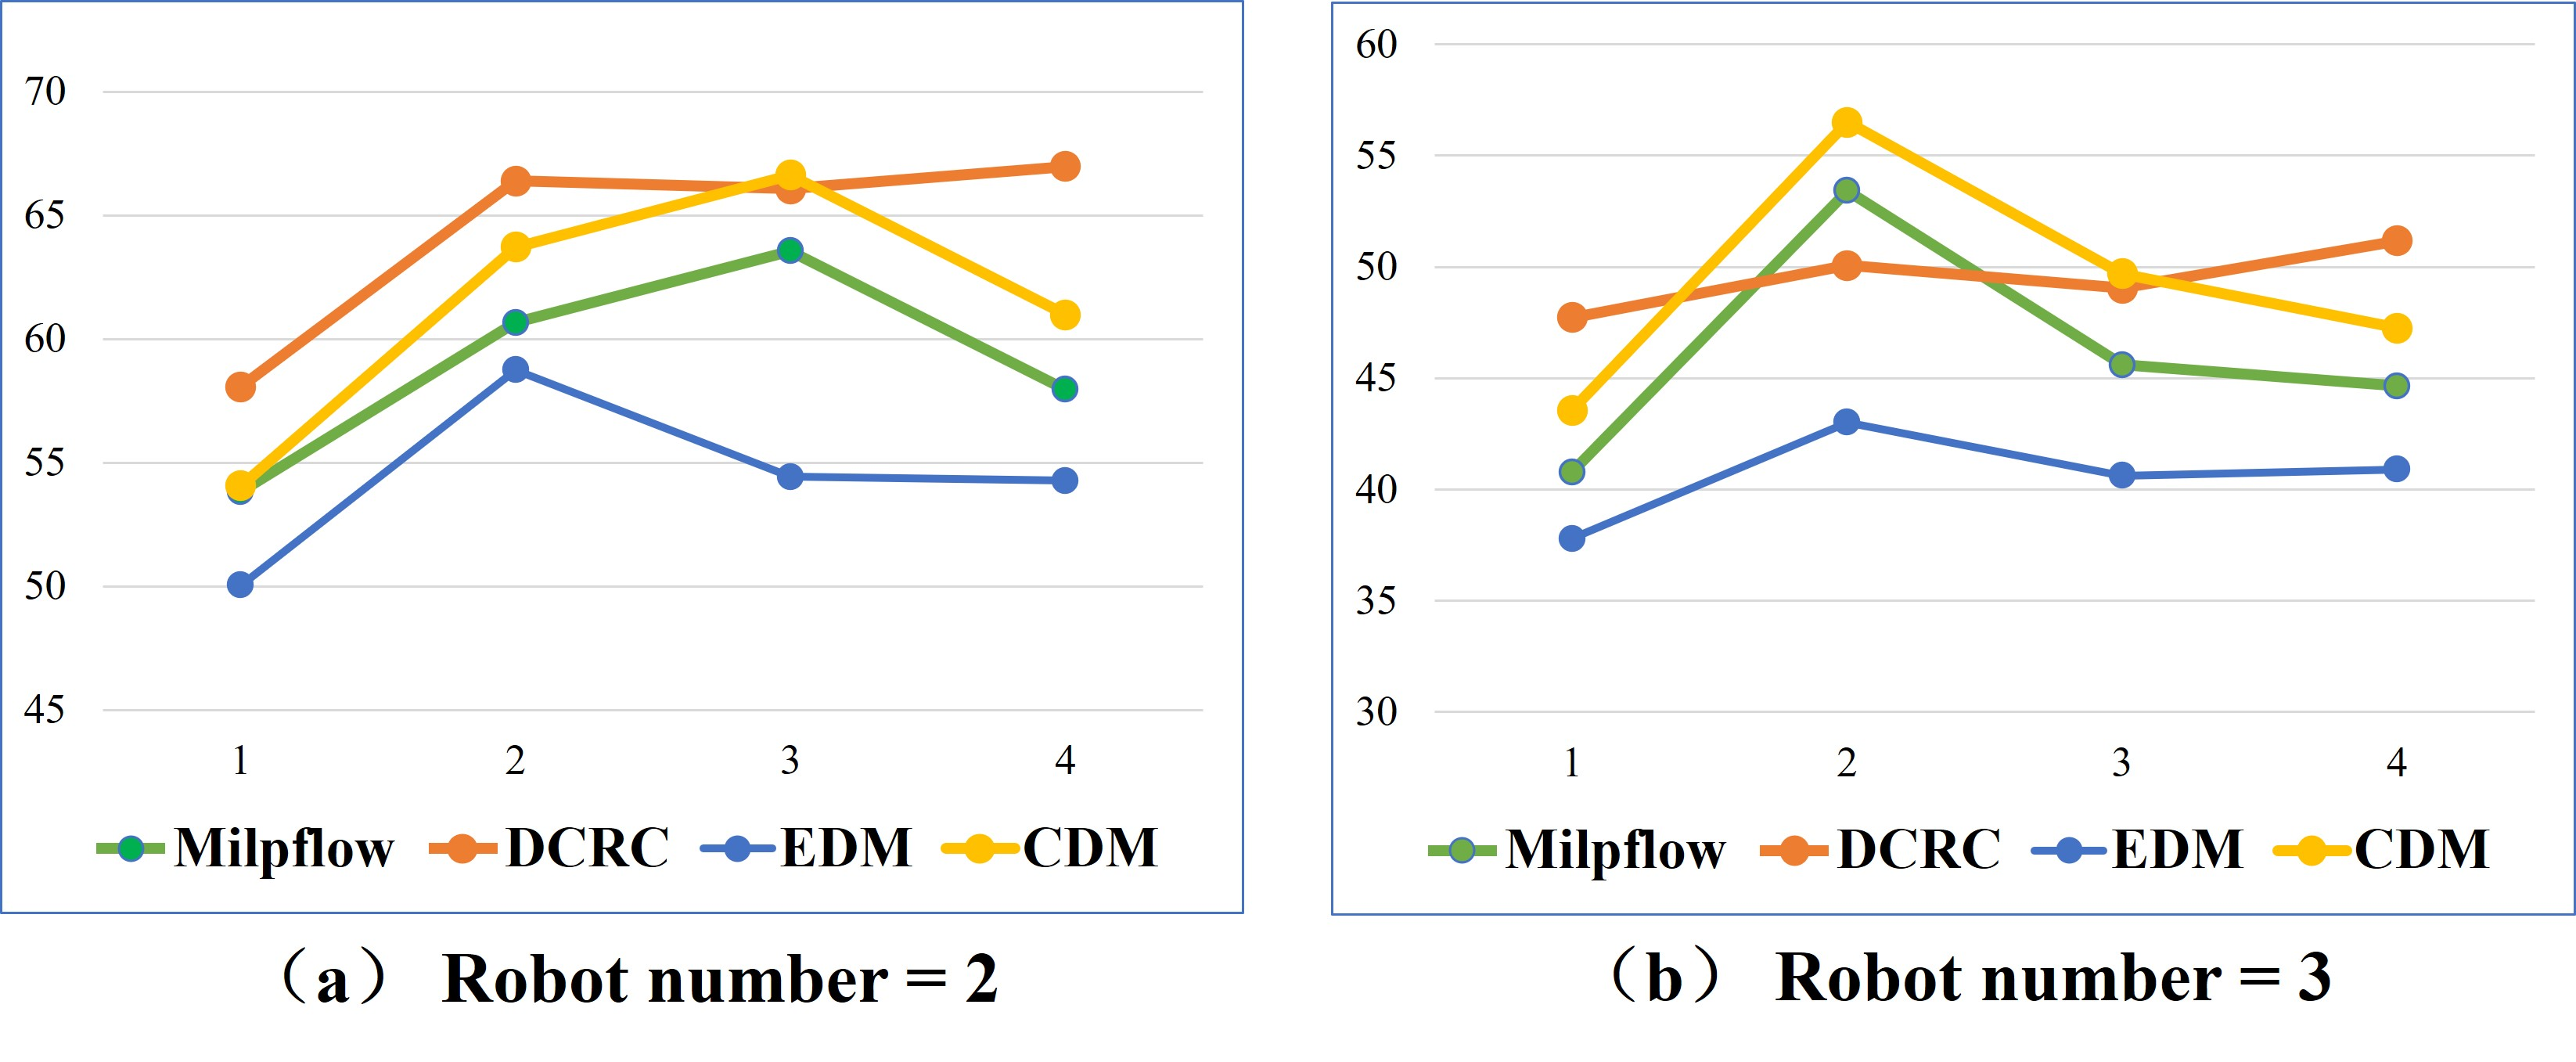
\includegraphics[width=0.75\textwidth]{8c.jpg}
    \caption{ The comparison of coverage times of Milpflow \cite{c39}, DCRC \cite{karapetyan2018multi}, \replaced{EDM}{EMD}, and \replaced{CDM}{CMD}. Fewer coverage times are better. }
    %\vspace{-0.4 cm} %设置与下面正文的距离
   \label{Fig_8c}
\end{figure}

A variety of experiments were performed using teams of two or three robots on different maps. Fig.\ref{Fig_8a} and \ref{Fig_8b} demonstrate snapshots of coverage paths produced by Milpflow \cite{c39}, DCRC \cite{karapetyan2018multi}, \replaced{EDM}{EMD}, and \replaced{CDM}{CMD}, respectively. These snapshots show that \replaced{Milpflow and CDM produce relatively concentrated paths for every robot since they allocate a set of connected coverage cells to every robot. In contrast to Milpflow and CDM, EDM and DCRC generate the single-robot coverage path that is not limited in a particular area.}{a single robot has a relatively concentrated coverage path in the Milpflow and CMD algorithms since they divide the region into subareas and then apply a single-robot Dubins solver to each subarea. The DCRC algorithm generates $K$ coverage paths by splitting the single-robot tour into $K$ subtours, while EMD optimizes the MILP to produce optimal coverage paths. Thus, their single-robot coverage paths are not clustered in specific areas.}



%These snapshots show that both Milpflow and CMD algorithms produces the relatively concentrated coverage paths for a single robot, since they divide the region into subareas and apply a single-robot Dubins solver to each subarea. By contrast, EMD optimizes the DMCPP problem from a global perspective rather than breaking it into subproblems. Thus, its coverage paths are not clustered in the specific areas.

Fig.\ref{Fig_8c} compares coverage times of Milpflow \cite{c39}, DCRC \cite{karapetyan2018multi}, \replaced{EDM}{EMD}, and \replaced{CDM}{CMD}, respectively. \replaced{The comparison results show that, compared with heuristic DCRC and CDM, Milpflow and EDM provide fewer coverage times by thoroughly searching the solution space. Furthermore, EDM produces the least coverage times in all scenes because it generates the optimal Dubins coverage path rather than the area division provided by Milpflow.}{The comparison results show that EMD provides the least coverage time than other exact or heuristic coverage algorithms. However, EMD takes more runtime than the other three algorithms since it has a large search space.}

\subsection{Comparison experiments in large scenes}

In order to evaluate the performance of the proposed algorithm, a variant of the well-known environments from \cite{c46} was used. As shown in Fig.\ref{Fig_9}, the maps differ in terms of sizes and shapes. A set of experiments were conducted with teams of $\{3,6,9,12\}$ robots. Since Milpflow and \replaced{EDM}{EMD} cannot provide efficient solutions within limited time, this subsection only evaluates the heuristic \replaced{CDM}{CMD} and DCRC \cite{karapetyan2018multi} algorithms. Two metrics are used for performance evaluation as follows:(i) \textit{ coverage time}, and (ii) \textit{ computation time}.

\begin{figure}[htbp] %这里使用的是强制位置,除非真的放不下,不然就是写在哪里图就放在哪里,不会乱动
	\centering  %图片全局居中
    \vspace{0 cm} %设置与上面正文的距离
    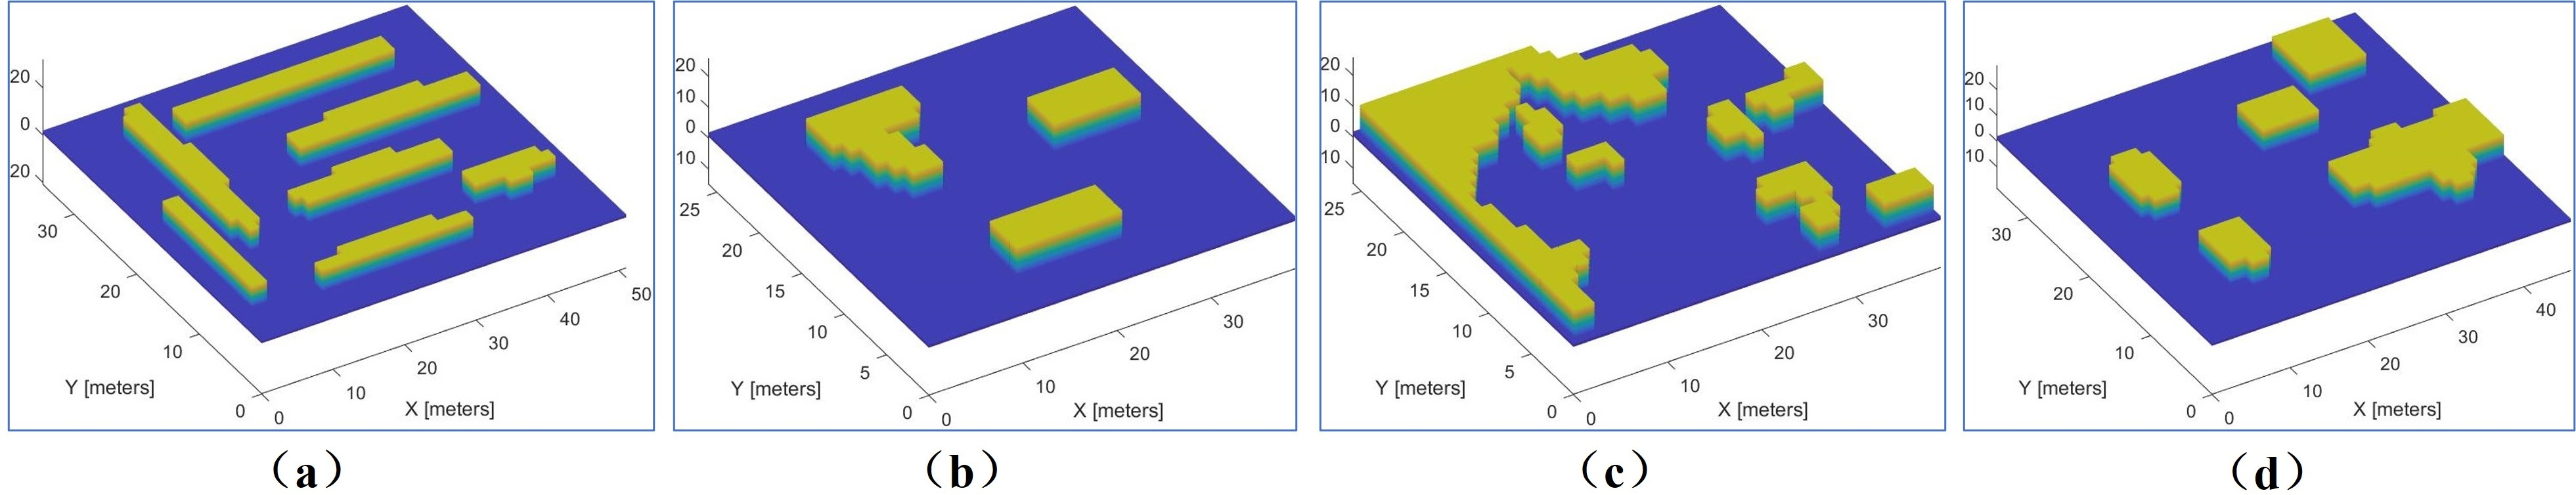
\includegraphics[width=0.98\textwidth]{9.jpg}
    \caption{ Four point cloud maps where \replaced{CDM}{CMD} and DCRC were tested. (a) Multi-cell(34 m $\times$ 50 m $\times$ 10 m); (b) Farm(25 $\times$ 38 m $\times$ 10 m); (c) Rural Quebec(25 m $\times$ 38 m $\times$ 10 m); (d) Cave(34 m $\times$ 45 m $\times$ 10 m);}
    %\vspace{-0.4 cm} %设置与下面正文的距离
   \label{Fig_9}
\end{figure}

\added{Fig.\ref{Fig_9a} and \ref{Fig_9b} demonstrate snapshots of coverage paths generated by DCRC and CDM for 3 and 6 robots, respectively. These snapshots show that the CDM algorithm provides a set of connected cells for every robot, while a single robot's coverage cells in DCRC may be disconnected. Paths between disconnected cells probably revisit the covered area, which increases the coverage time. Indeed, as illustrated in Fig.\ref{Fig_9c}, the CDM algorithm provides fewer coverage times than DCRC in most experiments.}

Fig.\ref{Fig_9d} shows the computation times of \replaced{CDM}{CMD} and DCRC with $\{3,6,9,12\}$ robots, respectively. It is observed that DCRC provides a approximately equal computation time in each scene, while the computation time of \replaced{CDM}{CMD} decreases with the increase of robot number. The difference in computation time between \replaced{CDM}{CMD} and DCRC derives from the search space. The larger the search space, the longer the computation time of the algorithm. DCRC plans a single-robot coverage path in terms of the entire map, which corresponds to a large search space. In contrast, \replaced{CDM}{CMD} divides the map into $K$ subareas and plans the path for each subarea. Compared with the entire map, subareas corresponds to a small search space. With the increase in robot number, \replaced{CDM}{CMD}'s computation times become smaller.

\deleted{Fig.\ref{Fig_9a} and \ref{Fig_9b} demonstrate snapshots of coverage paths generated by DCRC and \replaced{CDM}{CMD} for 3 and 6 robots, respectively. DCRC divides the single-robot optimal route into $K$ subpaths, each corresponding to a robot. As shown in the first row of Fig.\ref{Fig_9a} and \ref{Fig_9b}, crossings between subpaths occur in DCRC. In contrast, \replaced{CDM}{CMD} divides the map into $K$ subareas and employs the single-robot Dubins solver  \cite{c25} for each subarea. Thus, each robot's coverage path is clustered within its subarea.}


\begin{figure}[htbp] %这里使用的是强制位置,除非真的放不下,不然就是写在哪里图就放在哪里,不会乱动
	\centering  %图片全局居中
    \vspace{0 cm} %设置与上面正文的距离
    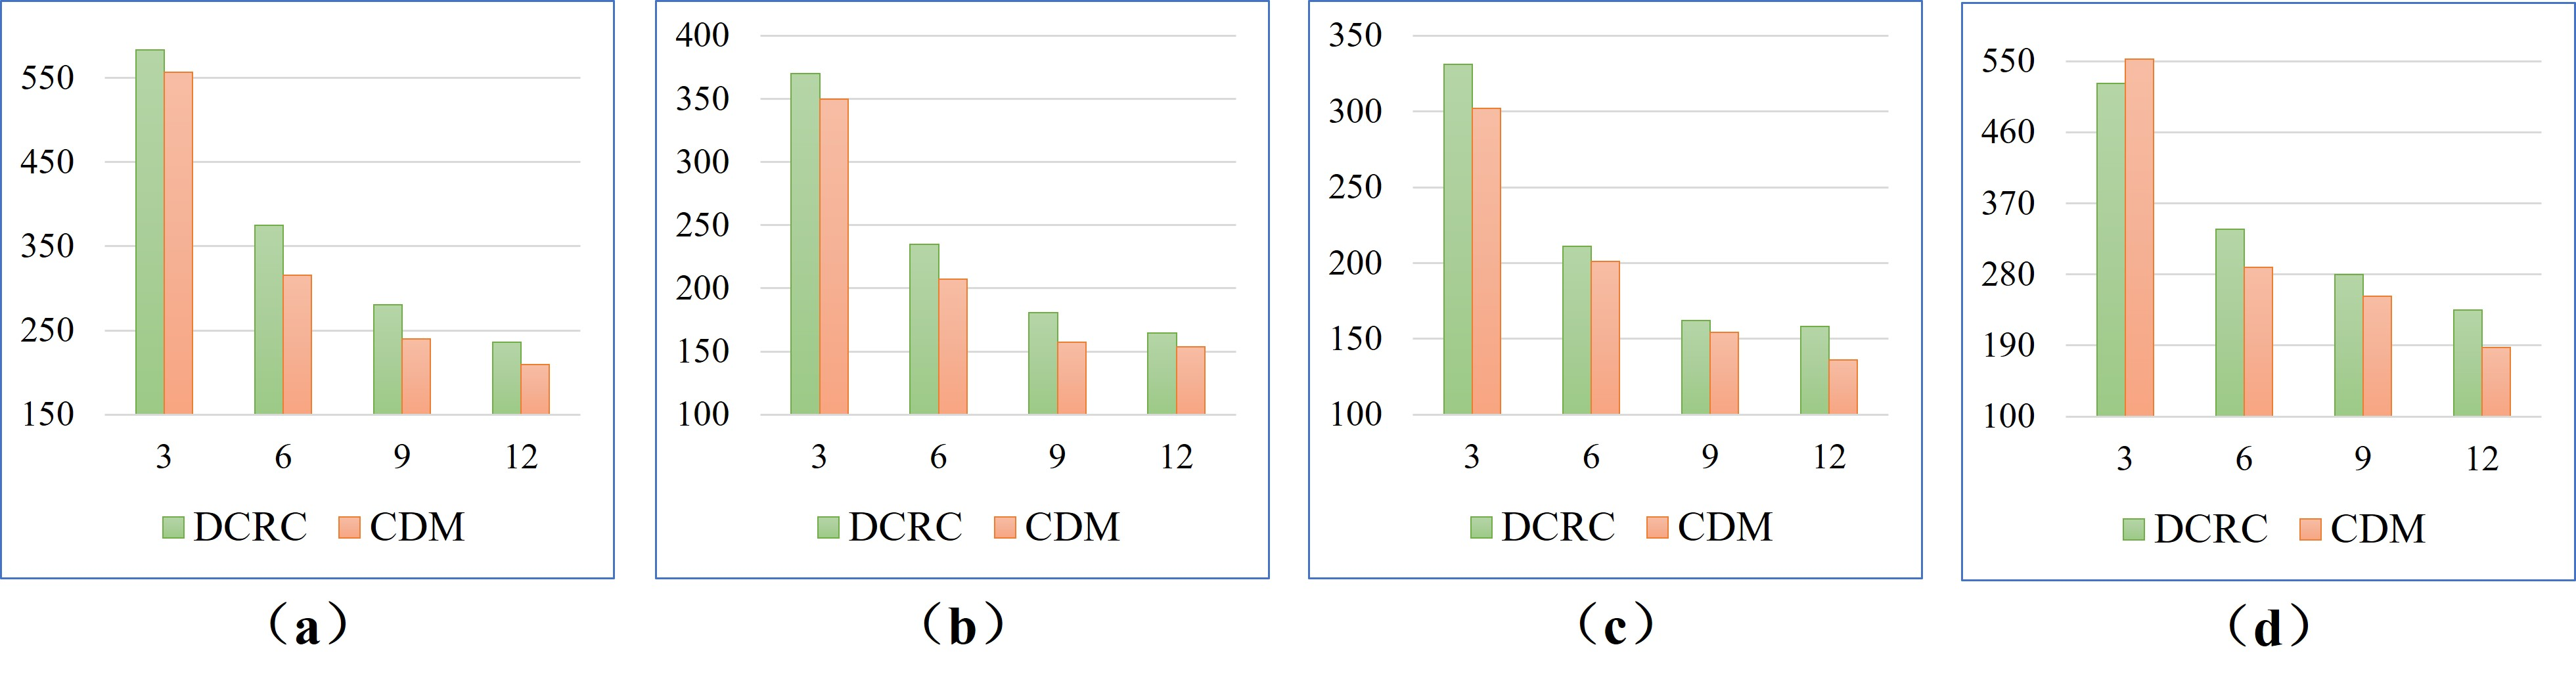
\includegraphics[width=0.98\textwidth]{coverage_time.jpg}
    \caption{ The comparison of coverage times for four different environments. Less coverage times are better.}
    %\vspace{-0.4 cm} %设置与下面正文的距离
   \label{Fig_9c}
\end{figure}

\begin{figure}[htbp] %这里使用的是强制位置,除非真的放不下,不然就是写在哪里图就放在哪里,不会乱动
	\centering  %图片全局居中
    \vspace{0 cm} %设置与上面正文的距离
    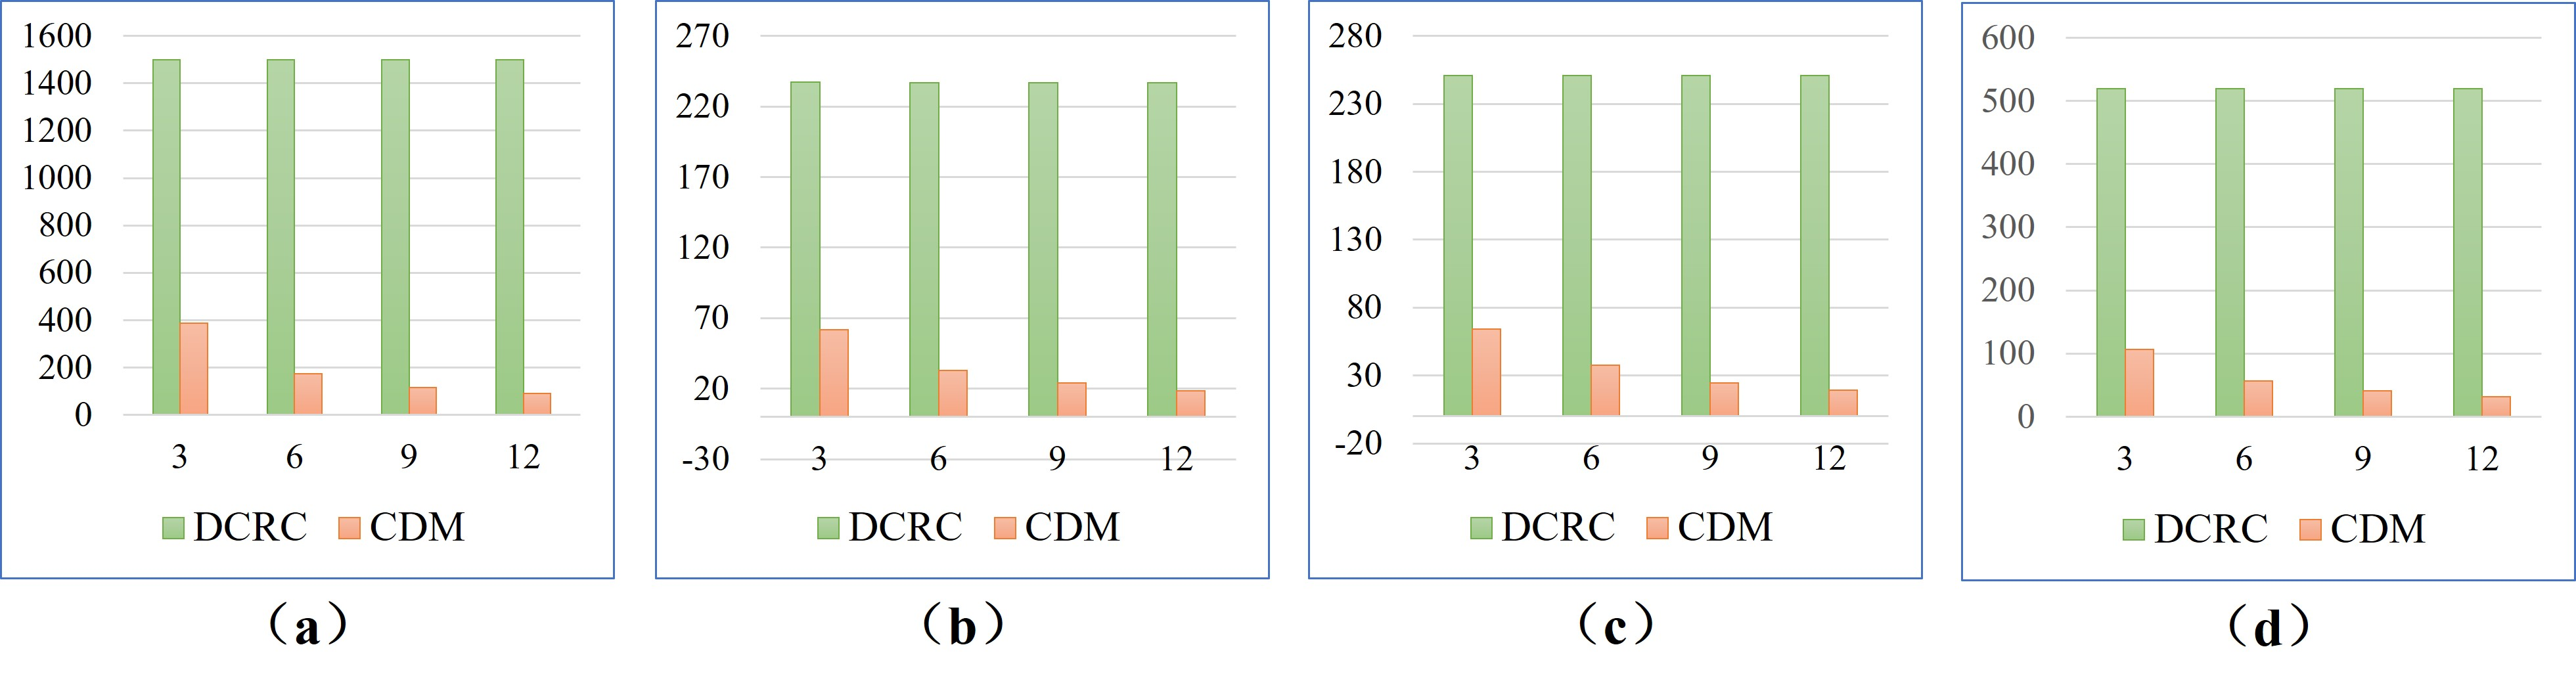
\includegraphics[width=0.98\textwidth]{computation_time.jpg}
    \caption{  The comparison of computation times for four different environments. Less computation times are better.}
    %\vspace{-0.4 cm} %设置与下面正文的距离
   \label{Fig_9d}
\end{figure}

\begin{figure}[htbp] %这里使用的是强制位置,除非真的放不下,不然就是写在哪里图就放在哪里,不会乱动
	\centering  %图片全局居中
    \vspace{0 cm} %设置与上面正文的距离
    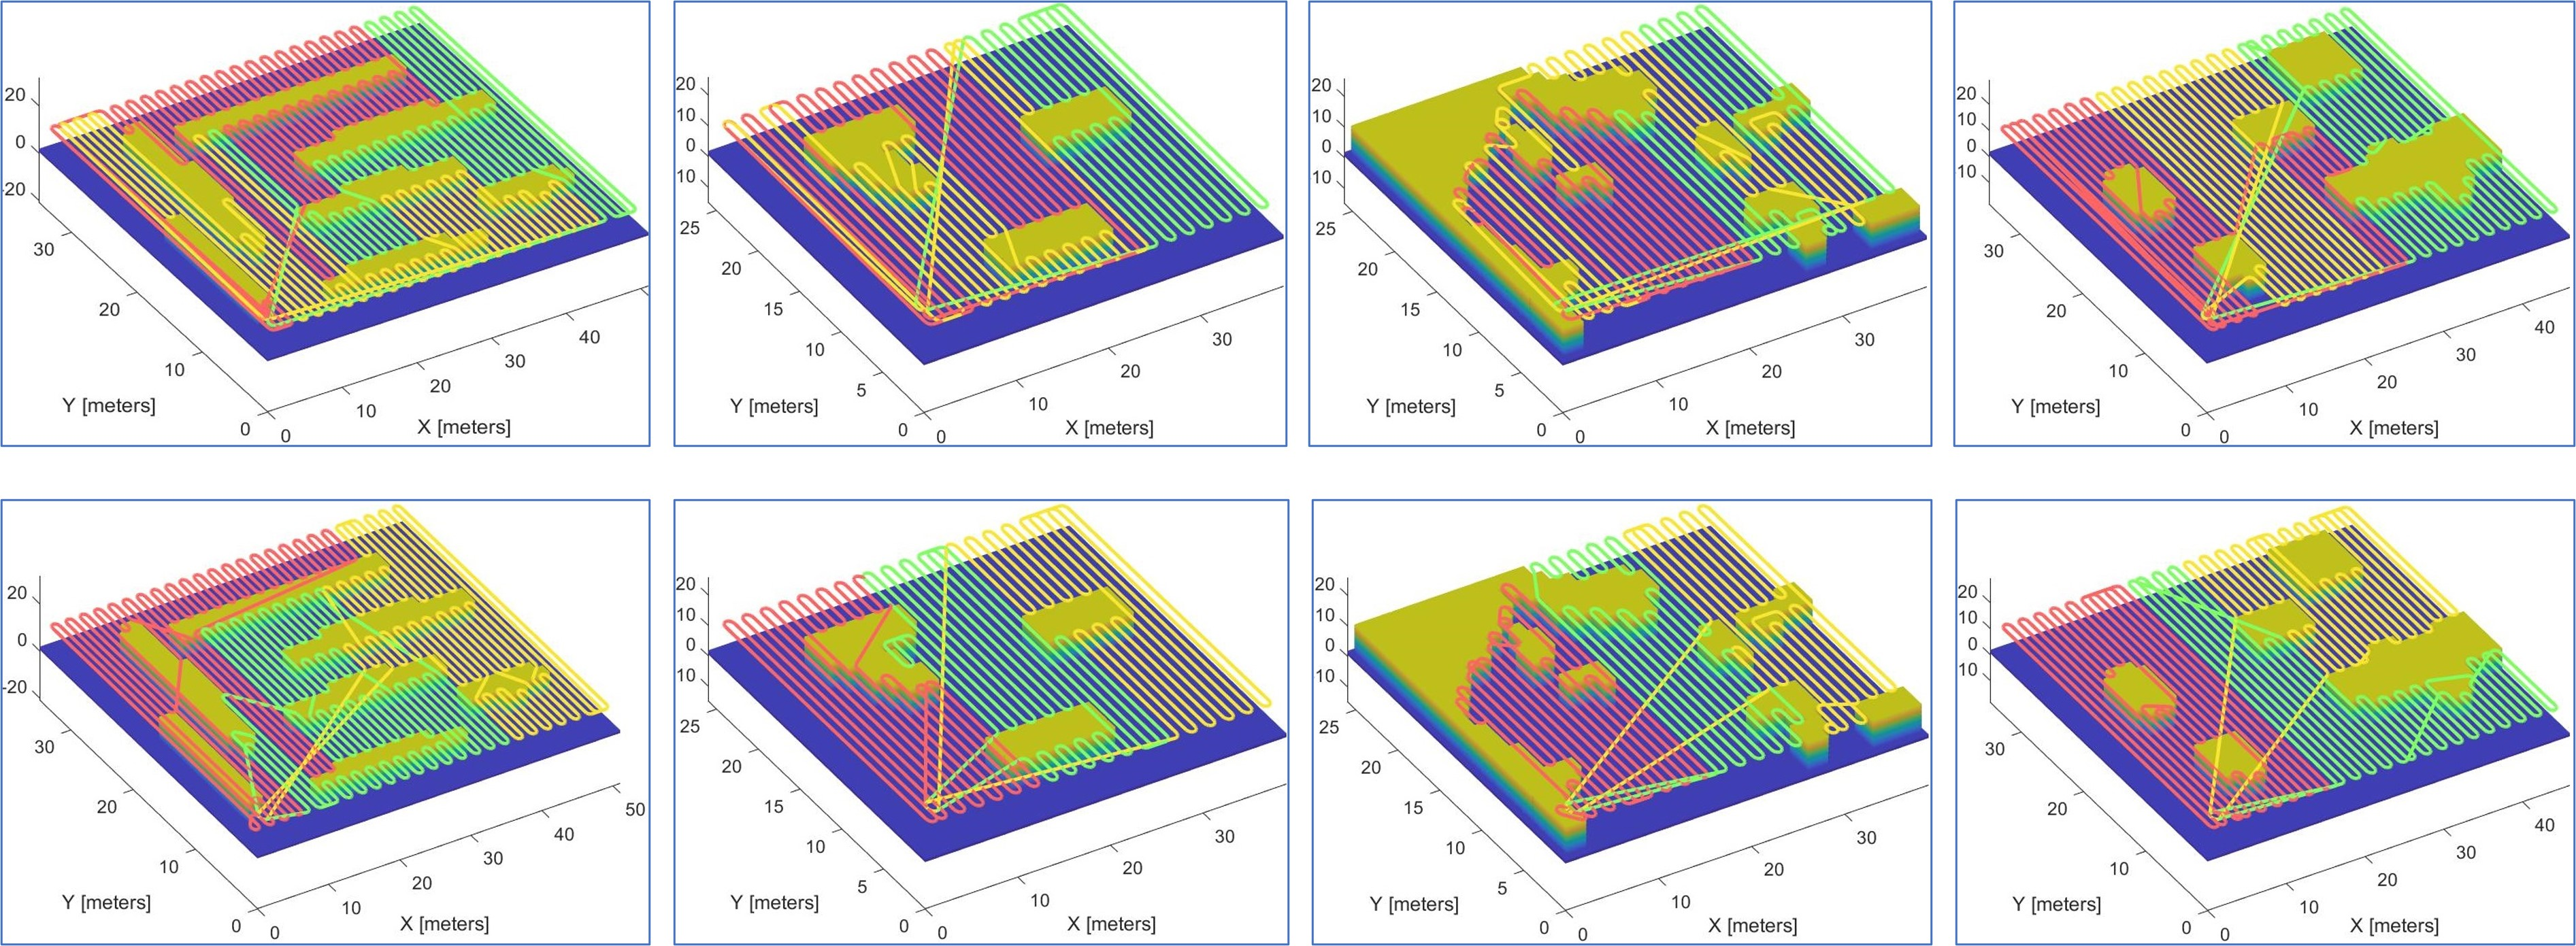
\includegraphics[width=0.98\textwidth]{9a.jpg}
    \caption{ Coverage paths of DCRC (first row) and \replaced{CDM}{CMD} (second row) with 3 robots.}
    %\vspace{-0.4 cm} %设置与下面正文的距离
   \label{Fig_9a}
\end{figure}

\begin{figure}[htbp] %这里使用的是强制位置,除非真的放不下,不然就是写在哪里图就放在哪里,不会乱动
	\centering  %图片全局居中
    \vspace{0 cm} %设置与上面正文的距离
    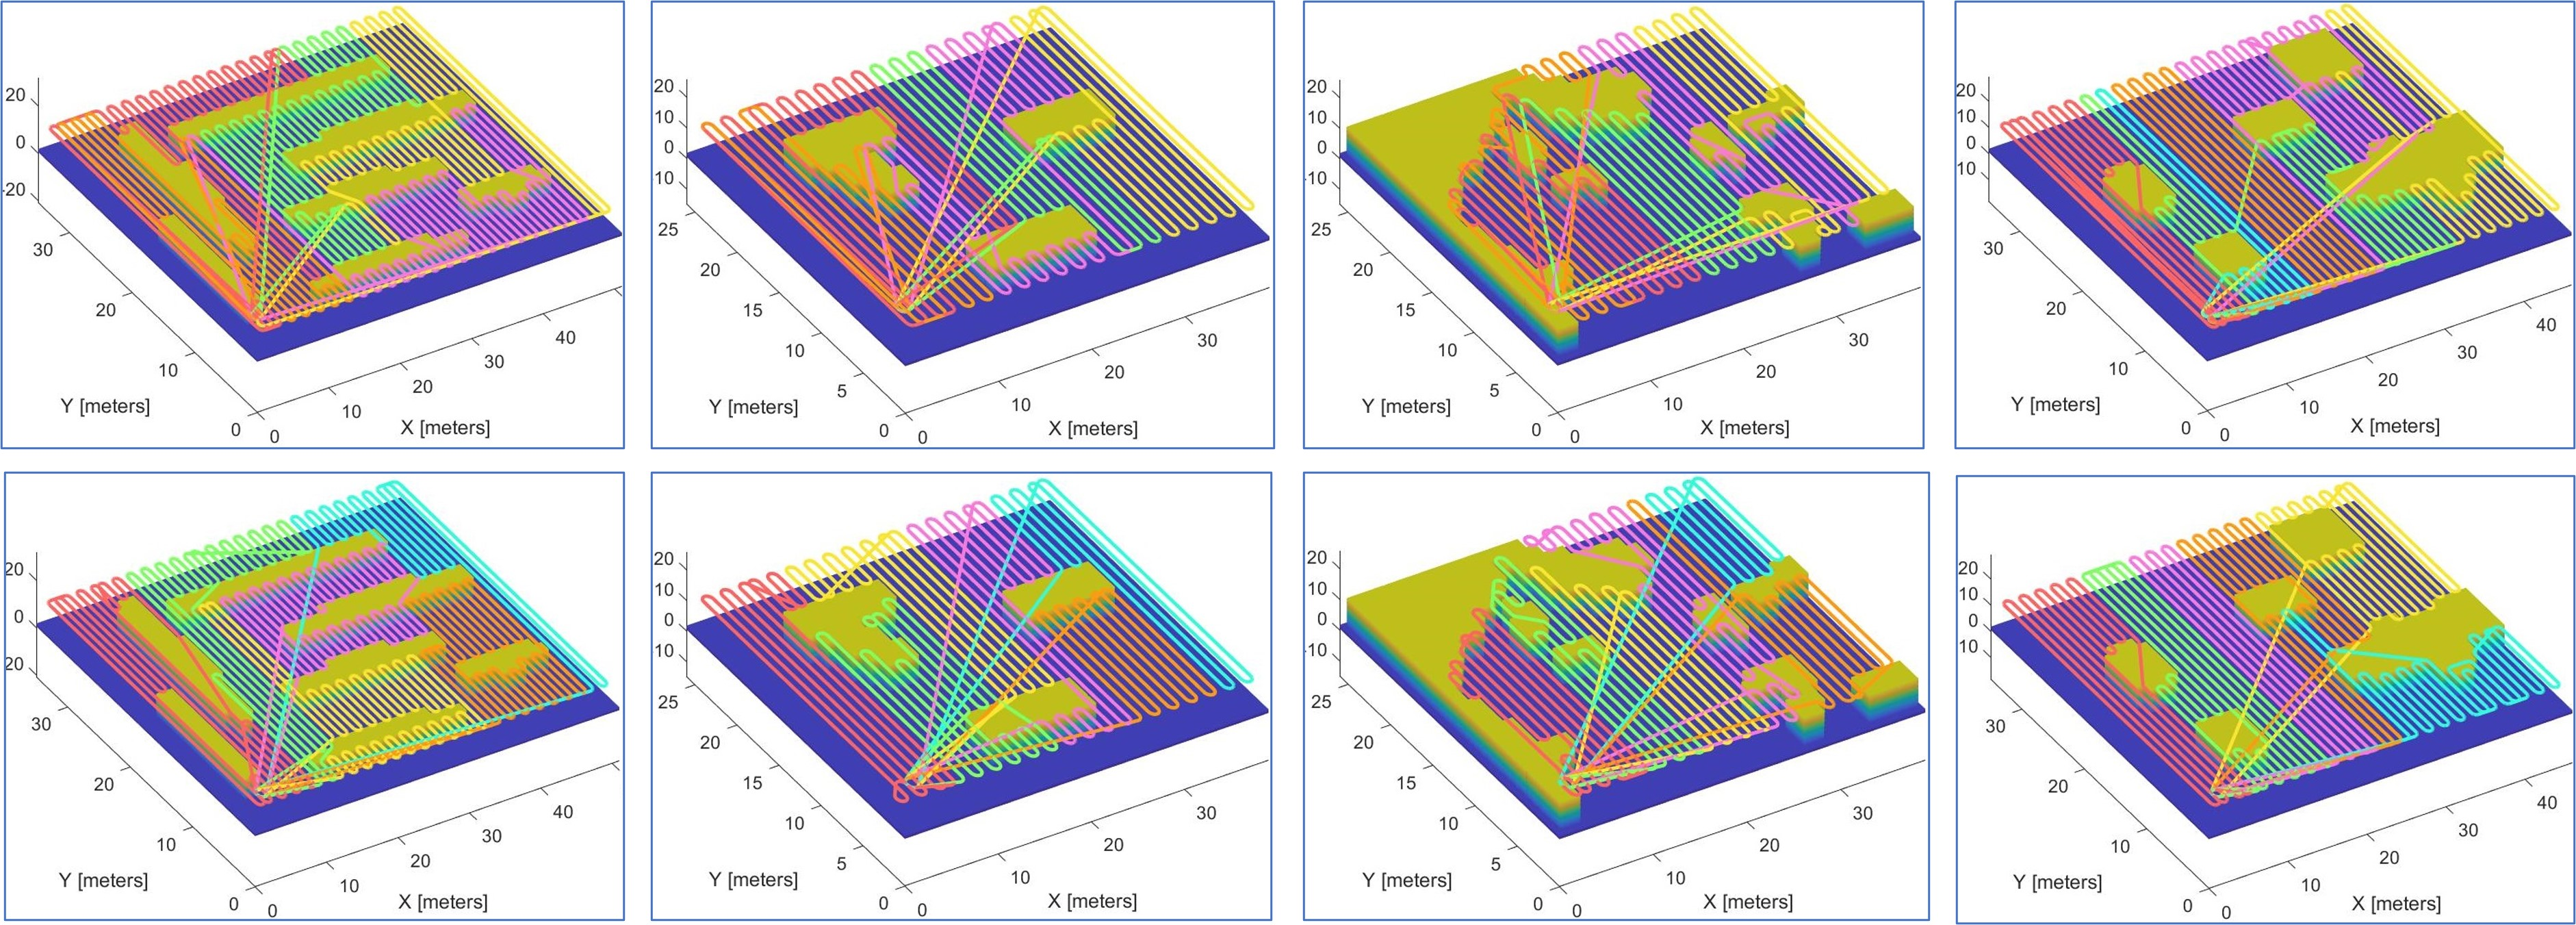
\includegraphics[width=0.98\textwidth]{9b.jpg}
    \caption{ Coverage paths of DCRC (first row) and \replaced{CDM}{CMD} (second row) with 6 robots.}
    %\vspace{-0.4 cm} %设置与下面正文的距离
   \label{Fig_9b}
\end{figure}


\subsection{Feasibility experiments of \replaced{EDM}{EMD} and \replaced{CDM}{CMD} }

We validate \replaced{EDM}{EMD} and \replaced{CDM}{CMD} algorithms with a high-fidelity fixed-wing UAV model \cite{UAVsimulated} in Simulink. A waypoint follower is integrated into the fixed-wing UAV model, which calculates the desired heading based on the current pose, look-ahead distance, and coverage paths. Experiments were conducted on UAVs with kinematic constraints such as 0.5m turning radius and 1 m/s speed. Each UAV was set at a different flight height to ensure its safety. Fig.\ref{Fig_11b} and \ref{Fig_12} demonstrate snapshots of the simulated UAV paths for \replaced{EDM}{EMD} and \replaced{CDM}{CMD} , respectively. The snapshots show that \replaced{EDM}{EMD} and \replaced{CDM}{CMD} are applicable to fixed-wing UAVs.

\begin{figure}[htbp] %这里使用的是强制位置,除非真的放不下,不然就是写在哪里图就放在哪里,不会乱动
	\centering  %图片全局居中
    \vspace{0 cm} %设置与上面正文的距离
    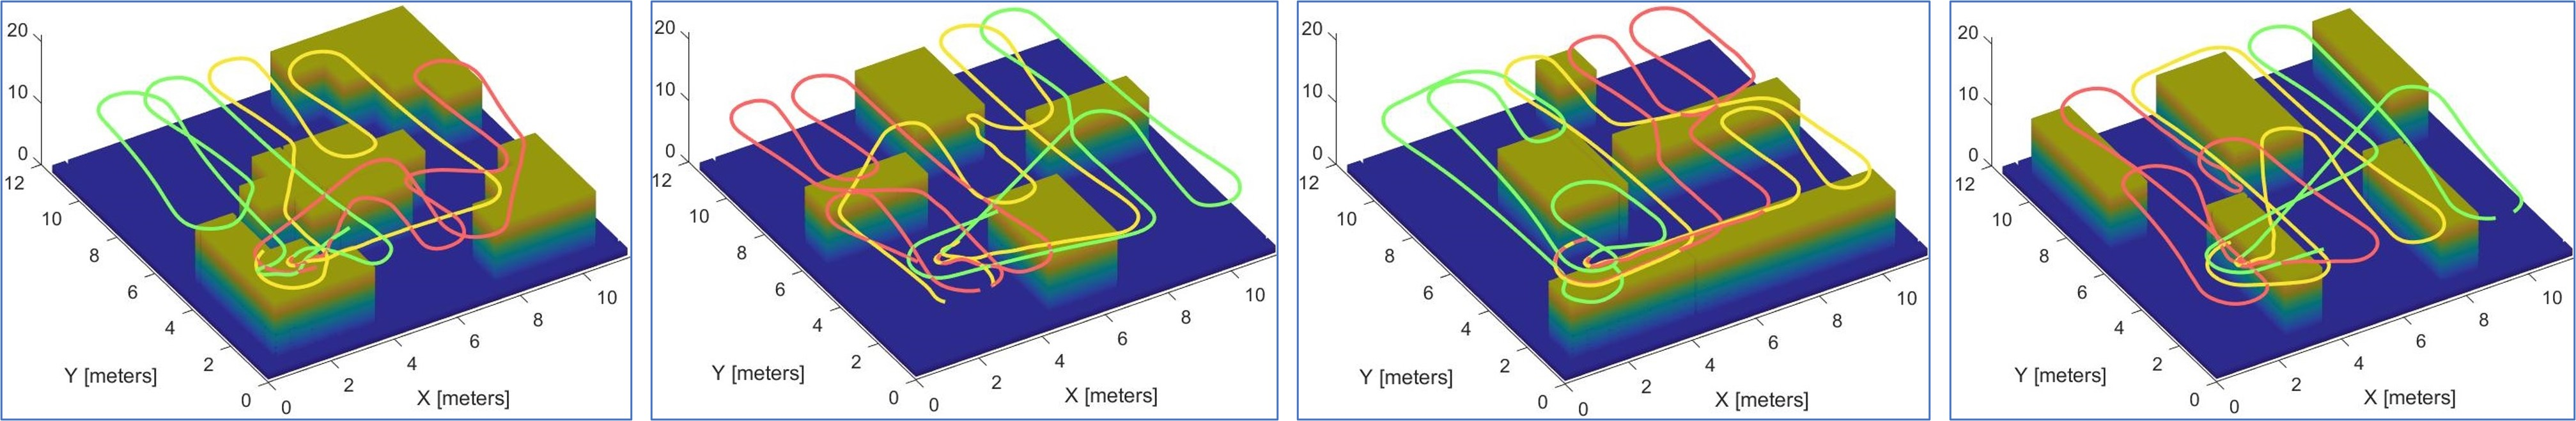
\includegraphics[width=0.98\textwidth]{11b.jpg}
    \caption{ UAV simulated paths of \replaced{EDM}{EMD} with 3 robots.}
    %\vspace{-0.4 cm} %设置与下面正文的距离
   \label{Fig_11b}
\end{figure}

\begin{figure}[htbp] %这里使用的是强制位置,除非真的放不下,不然就是写在哪里图就放在哪里,不会乱动
	\centering  %图片全局居中
    \vspace{0 cm} %设置与上面正文的距离
    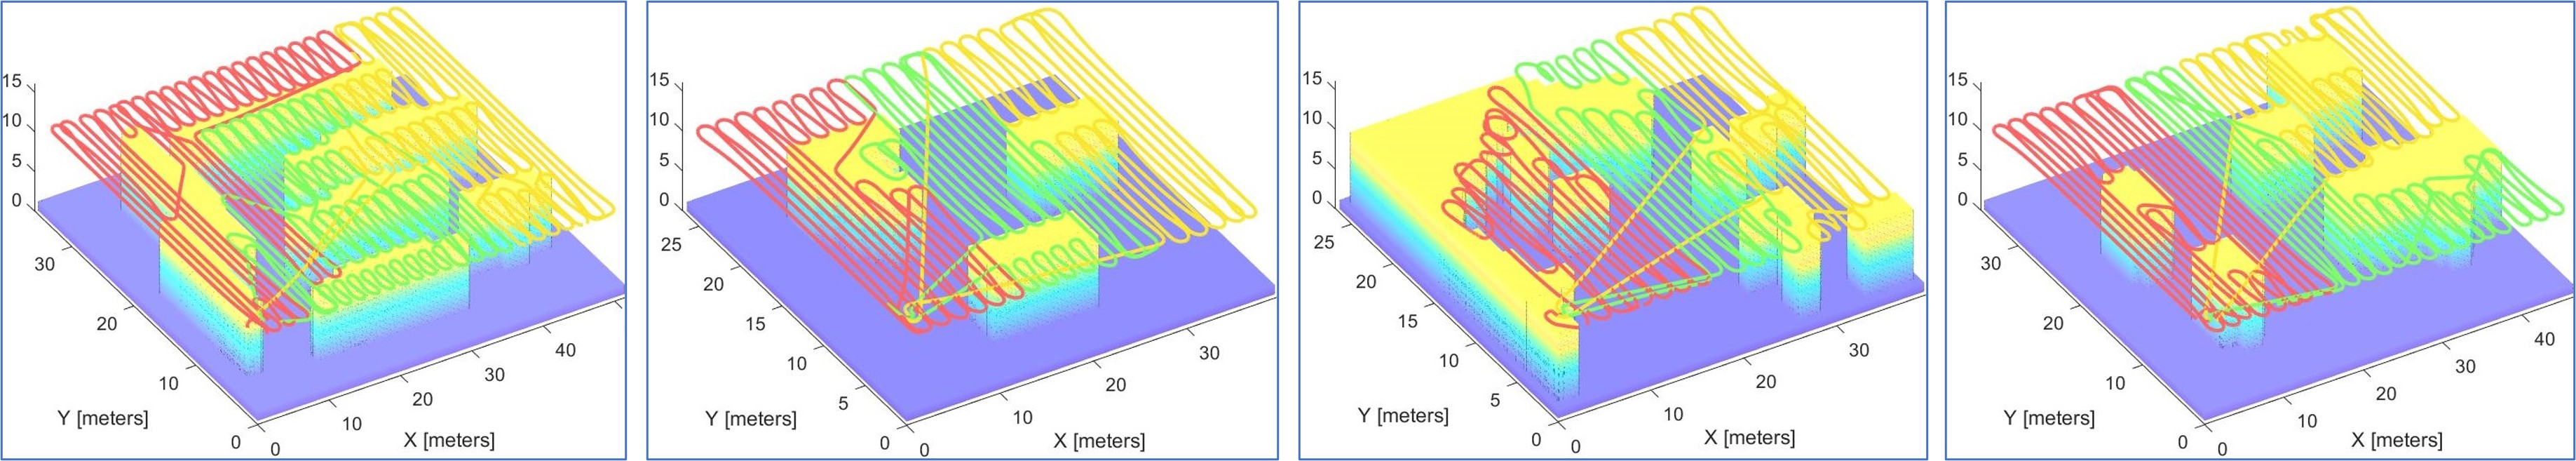
\includegraphics[width=0.98\textwidth]{12.jpg}
    \caption{ UAV simulated paths of \replaced{CDM}{CMD} with 3 robots.}
    %\vspace{-0.4 cm} %设置与下面正文的距离
   \label{Fig_12}
\end{figure}

\section{Conclusion}
\label{Sec_Conclusion}

This paper presents an \replaced{EDM}{exact EMD} algorithm and a heuristic \replaced{CDM}{CMD} algorithm to address the \replaced{Dubins MCPP}{DMCPP} problem. \replaced{EDM}{EMD} formulates the \replaced{Dubins MCPP}{DMCPP} problem into a MILP to produce the shortest Dubins coverage paths. \replaced{CDM}{CMD} balances the coverage tasks among robots by a credit model and reduces the complexity of the \replaced{Dubins MCPP}{DMCPP} problem by a tree partition strategy, providing an approximate optimal solution. \replaced{It is shown that both EDM and CDM can provide smooth and continuous Dubins coverage paths. Comparison experiments with other exact or heuristic algorithms demonstrate that EDM produces the fastest Dubins coverage path in small-scale scenes, and CDM produces less coverage time and shorter computation time than other heuristic algorithms in large-scale scenes. Feasibility experiments show that the results from the simulations and the analysis performed on those results hold for high-fidelity Dubins robotic systems.}{EMD and CMD were validated in comparison experiments with other exact and approximate algorithms. The comparison results show that EMD provides the least coverage time in small-scale scenes, while CMD produces less coverage time and shorter computation time in large-scale scenes. In addition, the applicability of EMD and CMD was validated via high-fidelity simulations for fixed-wing UAVs.} Future research areas include: (i) extending online coverage to unknown environments, (ii) applying to real Dubins robots.

\paragraph{\textbf{Author Contributions:} The work presented here was carried out in collaboration among all authors. All authors have contributed to, seen and approved the manuscript.}
%Conceptualization, Songchang Jin, Shaowu Yang, Chenlei Zhou and HengZhu Liu; Formal analysis, Lin Li, Dianxi Shi, Songchang Jin and HengZhu Liu; Investigation, Lin Li; Methodology, Lin Li, Dianxi Shi, Songchang Jin, Shaowu Yang, Chenlei Zhou and HengZhu Liu; Project administration, Dianxi Shi and Shaowu Yang; Software, Lin Li and Yaoning Lian; Validation, Lin Li, Chenlei Zhou and Yaoning Lian; Writing – original draft, Lin Li; Writing – review & editing, Lin Li, Dianxi Shi and Songchang Jin.
\paragraph{\textbf{Acknowledgments:} This work was supported by Science and Technology Innovation 2030 Major Project under Grant No.2020AAA0104802. The work was also supported by National Natural Science Foundation of China (Grant No. 91948303). The authors would like to thank the anonymous reviewers for their valuable suggestions and providing many possible directions for the future work.}

\paragraph{\textbf{Conflicts of Interest:} The authors declare no conflict of interest.}

%%%%%%%%%%%%%%%%%%%%%%%%%%%%%%%%%%%%%%%%%%
\vspace{6pt}


%%%%%%%%%%%%%%%%%%%%%%%%%%%%%%%%%%%%%%%%%%
\begin{adjustwidth}{-\extralength}{0cm}
%\printendnotes[custom] % Un-comment to print a list of endnotes


\reftitle{References}

% Please provide either the correct journal abbreviation (e.g. according to the “List of Title Word Abbreviations” http://www.issn.org/services/online-services/access-to-the-ltwa/) or the full name of the journal.
% Citations and References in Supplementary files are permitted provided that they also appear in the reference list here.

%=====================================
% References, variant A: external bibliography
%=====================================
%\bibliography{your_external_BibTeX_file}

%=====================================
% References, variant B: internal bibliography
%=====================================
%\begin{thebibliography}{999}
% Reference 1
%\bibitem[Author1(year)]{ref-journal}
%Author~1, T. The title of the cited article. {\em Journal Abbreviation} {\bf 2008}, {\em 10}, 142--149.

%\end{thebibliography}

% If authors have biography, please use the format below
%\section*{Short Biography of Authors}
%\bio
%{\raisebox{-0.35cm}{\includegraphics[width=3.5cm,height=5.3cm,clip,keepaspectratio]{Definitions/author1.pdf}}}
%{\textbf{Firstname Lastname} Biography of first author}
%
%\bio
%{\raisebox{-0.35cm}{\includegraphics[width=3.5cm,height=5.3cm,clip,keepaspectratio]{Definitions/author2.jpg}}}
%{\textbf{Firstname Lastname} Biography of second author}

% For the MDPI journals use author-date citation, please follow the formatting guidelines on http://www.mdpi.com/authors/references
% To cite two works by the same author: \citeauthor{ref-journal-1a} (\citeyear{ref-journal-1a}, \citeyear{ref-journal-1b}). This produces: Whittaker (1967, 1975)
% To cite two works by the same author with specific pages: \citeauthor{ref-journal-3a} (\citeyear{ref-journal-3a}, p. 328; \citeyear{ref-journal-3b}, p.475). This produces: Wong (1999, p. 328; 2000, p. 475)

%%%%%%%%%%%%%%%%%%%%%%%%%%%%%%%%%%%%%%%%%%
%% for journal Sci
%\reviewreports{\\
%Reviewer 1 comments and authors’ response\\
%Reviewer 2 comments and authors’ response\\
%Reviewer 3 comments and authors’ response
%}
%%%%%%%%%%%%%%%%%%%%%%%%%%%%%%%%%%%%%%%%%%
\bibliography{references}
\end{adjustwidth}

%\bibliography{references}
\end{document}

